\documentclass{article}

\usepackage{amsmath}
\usepackage{enumitem}
\usepackage{graphicx}
\usepackage{hyperref}
\usepackage{xcolor}
\usepackage{subcaption}
\usepackage{geometry}
\usepackage{pgfplots}
\usepackage{xepersian}

\settextfont{XB Kayhan}
\setmathdigitfont{Yas}
\setlatintextfont{Times Newer Roman}

\title{\vspace{-4cm} \textbf{پاسخ تمرینات سری سوم درس یادگیری ماشین}}
\author{محمدرضا غفرانی  ۴۰۰۱۳۱۰۷۶}
\date{\today}

\begin{document}

\maketitle

\subsection*{پرسش‌های تشریحی}

\subsubsection*{سوال یک}

\begin{enumerate}[label=\alph*)]
    \item این جمله در حالت کلی اشتباه است. در \lr{Kernel SVM} کرنل برای $N$ داده
    یک ماتریس به اندازه $N \times N$ است، در نتیجه تعداد پارامتر‌ها در این حالت به
    اندازه مجموعه دادگان وابسته بوده و در نتیجه مدل بدون پارامتر است. اما در \lr{Linear SVM} از آن جا که تعداد پارامتر‌ها تنها
    ،به ابعاد بردار ورودی بستگی دارد؛ بنابراین \lr{Linear SVM} یک مدل پارامتریک است.
    \item این جمله در حالت کلی درست است. از آنجا که \lr{SVM} سعی می‌کند خطی که بیشترین تمایز را در بین
    داده‌ها ایجاد می‌کند را پیدا می‌کند در نتیجه نسبت به بیش‌برازش نسبتا مقاوم است، البته طبق این \href{https://stats.stackexchange.com/a/35311/343311}{پاسخ}
    در عمل مقاوم بودن آن وابستگی زیادی به مقدار پارامتر $C$ دارد.
    \item درست است. در الگوریتم \lr{SVM} بردار‌های پشتیان هستند که سهم فراوانی در تعیین خط جداکننده دارند.
    اگر این بردار‌های پشتیبان شامل‌ داده‌های پرت باشند با مدیریت درست پارامتر $C$ می‌توان از تاثیر آن‌ها بر روی مدل نهایی جلوگیری کرد.
    \item نادرست است. الگوریتم \lr{adaboost} با ترکیب چندین درخت با عمق یک سعی می‌کند به بهترین
    مدل بر روی داده‌های آموزشی برسد. هر یک از این درخت‌ها به تنهایی یک دسته‌بند ضعیف هستند.
    \item نادرست است. می‌دانیم وزن‌های اختصاص داده شده به هر یک از دسته‌بند‌ها در این الگوریتم از رابطه
    $\ln\frac{1-e_i}{e_i}$ محاسبه می‌شود. در این فرمول اگر مقدار $e_i$ بزرگتر از $0.5$ و کم‌تر از یک
    باشد، در این صورت وزن داده شده یک مقدار مثبت است. اما اگر مقدار $e_i$ کمتر از $0.5$ و بزرگتر از
    صفر باشد وزن نسبت داده شده به درخت منفی خواهد بود. بدین معنی که این درخت دسته داده‌ها را به عکس پیش‌بینی می‌کند؛
    اگر کلاس داده مثبت باشد، درخت کلاس را منفی و اگر کلاس داده منفی باشد، درخت کلاس را مثبت پیش‌بینی می‌کند.
    \item درست است. در الگوریتم \lr{Adaboost} هر بار یک درخت با عمق یک ساخته می‌شود. از آن جا که این درخت قادر به
    پیش‌بینی درست تمام داده‌ها نیست، در نتیجه در هر مرحله به داده‌هایی که به اشتباه برچسب زده شده‌اند، اهمیت بیشتری
    داده می‌شود تا در مرحله بعدی الگوریتم به درستی برچسب زده شوند. حال اگر یک داده پرت در بین داده‌ها موجود باشد،
    با گذشت هر مرحله از الگوریتم وزن متناظر داده پرت بیشتر و بیشتر می‌شود و حتی ممکن است که الگوریتم تصمیم بگیرد
    یک درخت مجزا برای دسته‌بندی درست این داده در نظر بگیرد که از قضا درخت حاصل شده وزن زیادی هم داشته باشد.
\end{enumerate}

\subsection*{سوال دو}

\subsubsection*{قسمت الف}

بله با توجه به شکل \ref{q2-parta} داده‌ها جداپذیر خطی هستند.

\begin{figure}[h]
    \centering
    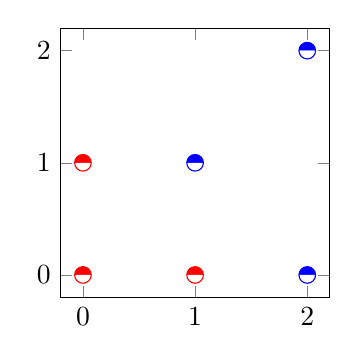
\begin{tikzpicture}
        \begin{axis}[width=5cm, height=5cm, scatter/classes={p={mark=halfcircle*, color=blue, mark size=3pt},n={mark=halfcircle*, color=red, mark size=3pt}}]
        \addplot[scatter,only marks, scatter src=explicit symbolic]
            table[meta=label] {
                x y label
                1 1 p
                2 2 p
                2 0 p
                0 0 n
                0 1 n
                1 0 n
            };
        \end{axis}
    \end{tikzpicture}
    \caption{شکل متناظر داده‌های سوال دو بخش الف}
    \label{q2-parta}
\end{figure}

\subsubsection*{قسمت ب}

با توجه به شکل \ref{q2-parta} مشخص است که نقاط $\begin{bmatrix}0\\ 1\end{bmatrix}$، $\begin{bmatrix}1\\ 0\end{bmatrix}$،
$\begin{bmatrix}2\\ 0\end{bmatrix}$ و $\begin{bmatrix}1\\ 1\end{bmatrix}$ بردار‌های پشتیبان هستند. می‌دانیم برای بردار‌های پشتیبان
رابطه‌ی زیر برقرار است.

$$y_i(w^Tx_i+b) - 1 = 0$$

بنابراین داریم. (داده‌های با رنگ قرمز را کلاس مثبت و داده‌های با رنگ آبی را کلاس منفی در نظر می‌گیریم.)

\begin{align*}
    \begin{cases}
        (w^T\begin{bmatrix}0\\ 1\end{bmatrix} + b) - 1 = 0\\\\
        (w^T\begin{bmatrix}1\\ 0\end{bmatrix} + b) - 1 = 0\\\\
        - (w^T\begin{bmatrix}2\\ 0\end{bmatrix} + b) - 1 = 0\\\\
        - (w^T\begin{bmatrix}1\\ 1\end{bmatrix} + b) - 1 = 0\\\\
    \end{cases}
\end{align*}

با جایگذاری $w=\begin{bmatrix}w_1\\w_2\end{bmatrix}$ و حل دستگاه معادله بالا داریم: $w_1=w_2=-2, b=3$. بنابراین
معادله خط جداکننده به صورت زیر حاصل می‌شود.

$$\begin{bmatrix}-2\\-2\end{bmatrix}^T x + 3 = 0$$

\subsubsection*{قسمت ج}

در این حالت با توجه به شکل \ref{q2-parta} نقاط $\begin{bmatrix}0\\ 1\end{bmatrix}$، $\begin{bmatrix}1\\ 0\end{bmatrix}$،
$\begin{bmatrix}2\\ 0\end{bmatrix}$ و $\begin{bmatrix}1\\ 1\end{bmatrix}$ بردار‌های پشتیبان هستند. با توجه به محل قرارگیری آن‌ها
حذف هر یک از بردار‌های پشتیبان تاثیری در تغییر اندازه حاشیه ندارد.

\subsubsection*{قسمت د}

گزاره بیان شده صحیح است. برای اثبات درستی آن از برهان خلف کمک می‌گیریم. فرض کنیم نمونه‌ای وجود داشته باشد که در آن
با حذف بردار پشتیبان اندازه حاشیه کاهش یابد. در این حالت اگر مجددا بخواهیم که این بردار پشتیبان را به مجموعه دادگان
مسئله اضافه کنیم، انتظار داریم که اندازه حاشیه به حالت قبلی خود بازگردد، بدین معنی که اندازه حاشیه بیشتر شود.
در صورتی که این عمل غیر قابل تصور است چرا که این داده جدید یا در حاشیه دسته‌بندی قرار دارد یا نه. اگر در حاشیه دسته‌بندی
قرار گیرد که اندازه حاشیه را کم‌تر می‌کند. در غیر این صورت نیز بردار خود بیش از حذف تاثیری در تعیین حاشیه نداشته است.
بنابراین استدلال فرض خلف باطل شده و حکم مسئله ثابت می‌شود.

\subsection*{سوال سه}

\subsubsection*{قسمت الف}

خیر، با توجه به نحوه قرارگیری داده‌های این سوال در شکل \ref{question3-parta}، داده‌ها جدا پذیر خطی نیستند.

\begin{figure}[h]
    \centering
    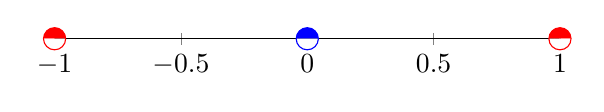
\begin{tikzpicture}
        \begin{axis}[axis x line=bottom, hide y axis, height=2cm, width=8cm, ymin=0,ymax=5, scatter/classes={p={mark=halfcircle*, color=blue, mark size=4pt},n={mark=halfcircle*, color=red, mark size=4pt}}]
        \addplot[scatter,only marks, scatter src=explicit symbolic]
            table[meta=label] {
                x y label
                0 0 p
                1 0 n
                -1 0 n
            };
        \end{axis}
    \end{tikzpicture}
    \caption{شکل مجموعه دادگان سوال سه قسمت الف}
    \label{question3-parta}
\end{figure}

\subsubsection*{قسمت ب}

با تبدیل داده‌ها مطابق این داده‌ها هر یک از داده‌های $0$، $1$ و $-1$ به ترتیب به بردار‌های
$\begin{bmatrix}1\\ 0\\ 0\end{bmatrix}$، $\begin{bmatrix}1\\ -\sqrt{2}\\ 1\end{bmatrix}$ و $\begin{bmatrix}1\\ \sqrt{2}\\ 1\end{bmatrix}$
تبدیل می‌شود. با رسم این داده‌ها در شکل سه‌بعدی متوجه می‌شویم که داده‌ها در این فضا جداپذیر خطی هستند.
با توجه به قرارگیری داده‌ها برای به دست آوردن بیشترین فاصله بین کلاس‌ها صفحه رسم شده باید عمود بر محور
$z$ باشد. بنابراین معادله صفحه جداکننده برابر خواهد بود با $z=0.5$. یا به بیان دقیق‌تر، معادله خط
جداکننده برابر خواهد بود با

$$\begin{bmatrix}0\\ 0\\ 2\end{bmatrix}x - 1 =0$$

در این حالت، معادله دسته‌بند پیشنهاد شده توسط الگوریتم \lr{SVM} برابر $x^2=\frac{1}{2}$ خواهد بود.

\begin{figure}[h]
    \centering
    \begin{tikzpicture}
        \begin{axis}[axis lines = middle, xlabel={x}, scatter/classes={p={mark=halfcircle*, color=blue, mark size=4pt},n={mark=halfcircle*, color=red, mark size=4pt}}]
        \addplot3 [scatter,only marks, scatter src=explicit symbolic]
            table[meta=label] {
                x y z label
                1 0 0 p
                1 -1.4 1 n
                1 1.4 1 n
            };
        \end{axis}
    \end{tikzpicture}
    \caption{شکل مجموعه دادگان سوال سه قسمت ب}
    \label{question3-partb}
\end{figure}

\subsection*{سوال چهار}

\begin{enumerate}[label=\alph*)]
    \item \textbf{\lr{SVM} خطی، \lr{soft margin}, $C=0.1$}: با توجه به صورت سوال جداکننده بین کلاس‌ها یک
    دسته‌بندی خطی است. این مورد تنها در شکل‌های ۳ و ۴ دیده می‌شود. با دقت در دو شکل ۳ و ۴ متوجه می‌شویم که
    تفاوت این دو در تعداد بردار‌های پشتیبان و نرخ خطای دسته‌بندی است. می‌دانیم با کم‌بودن $C$ مدل احتمال کم‌برازش بیشتری
    دارد. بنابراین شکل ۴ مربوط به بخش (الف) و شکل ۳ مربوط به بخش (ب) است.
    \item \textbf{\lr{SVM} خطی، \lr{soft margin}, $C=10$}: با توجه به توضیحات موجود در بند (آ) شکل ۳ مربوط به این
    دسته‌بند است.
    \item \textbf{\lr{hard margin SVM} با کرنل $u.v + (u.v)^2$}: با توجه به آن که این عبارت مجموع دو عبارت
    چند‌جمله‌ای است در نتیجه یک عبارت چندجمله‌ای بوده و شکل ۲ دسته‌بندی انجام شده توسط این دسته‌بند را نشان می‌دهد.
    \item \textbf{\lr{hard margin SVM} با کرنل $\text{\lr{exp}}(-\frac{1}{4}||u-v||^2)$}: می‌دانیم
    کرنل \lr{RBF} سعی می‌کند دسته‌ها را با استفاده از یک دایره مشخص کند. بنا بر این استدلال، یکی از شکل‌های
    ۱ یا ۶ نشان‌دهنده دسته‌بندی انجام شده توسط کرنل \lr{RBF} است. همچنین می‌دانیم اگر مقدار $\gamma$ کم باشد،
    دسته تولید شده نرم‌تر است اما اگر مقدار $\gamma$ زیاد باشد، تقریبا هر نقطه از داده به عنوان یک دسته انتخاب
    خواهد شد. در نتیجه شکل ۱ مربوط به دسته‌بند «\lr{hard margin SVM} با کرنل $\text{\lr{exp}}(-\frac{1}{4}||u-v||^2)$»
    و شکل ۶ مربوط به دسته‌بند «\lr{hard margin SVM} با کرنل $\text{\lr{exp}}(-4||u-v||^2)$» است.
    \item \textbf{\lr{hard margin SVM} با کرنل $\text{\lr{exp}}(-4||u-v||^2)$}: با توجه به توضیحات قسمت قبل
    دسته‌بندی انجام شده توسط این دسته‌بند در شکل ۶ رسم شده است.
\end{enumerate}

\subsection*{سوال پنجم}

با توجه به آن که $h_1$ تنها یکی از داده‌ها را به اشتباه برچسب زده است، در نتیجه مقدار $e_1$ برابر $\frac{1}{8}$
می‌شود. داده‌ای که $h_1$ برچسب آن را اشتباه تشخیص می‌دهد یکی از کلاس‌های مثبت است. در ادامه وزن متناظر این دسته‌بند را محاسبه
می‌کنیم. می‌دانیم وزن از رابطه زیر محاسبه می‌شود.

$$\alpha_i = \frac{1}{2} \ln\frac{1-e_i}{e_i}, \vee i$$

بنابراین داریم.

$$\alpha_1 = \frac{1}{2} \ln\frac{1-\frac{1}{8}}{\frac{1}{8}}=\frac{1}{2} \ln(7) \simeq 0.972$$

\newpage
\section*{سوال‌های پیاده‌سازی}

\subsection*{سوال یک}

\subsubsection*{قسمت الف}

در شکل \ref{sepal} و \ref{petal} به ترتیب نمودار متناظر کاسبرگ و گلبرگ هر یک از گونه‌ها مشاهده می‌شود. و

\begin{figure}[h]
    \begin{subfigure}{0.45\textwidth}
        \centering
        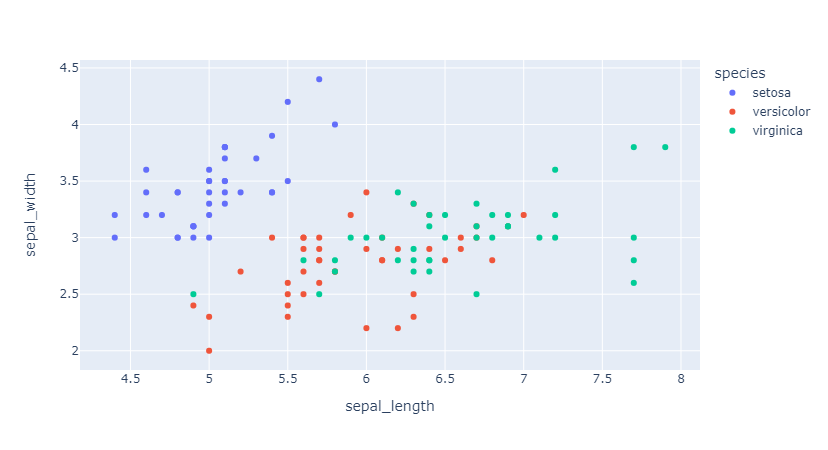
\includegraphics[scale=.15]{images/implementation/q1/sepal.png}
        \caption{نمودار طول کاسبرگ به عرض کاسبرگ}
        \label{sepal}
    \end{subfigure}
    \hfill
    \begin{subfigure}{0.45\textwidth}
        \centering
        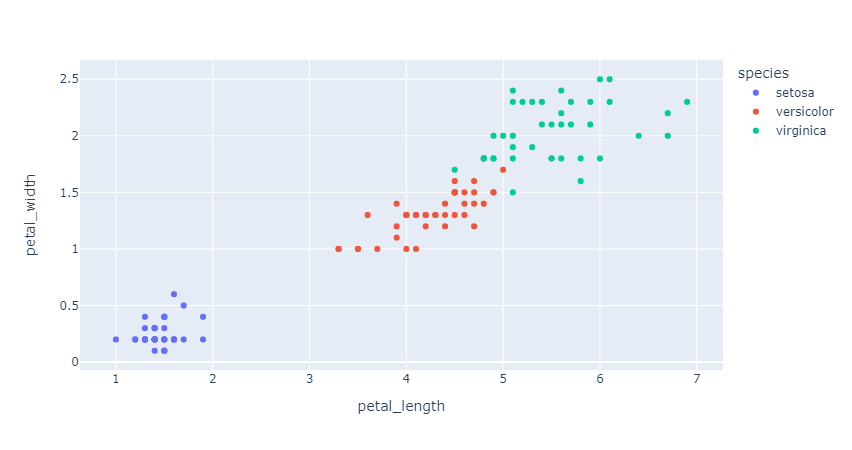
\includegraphics[scale=.15]{images/implementation/q1/petal.png}
        \caption{نمودار طول گلبرگ به عرض گلبرگ}
        \label{petal}
    \end{subfigure}
    \caption{نمودار طول و عرض کاسبرگ و گلبرگ هر یک گونه‌ها}
\end{figure}

\subsubsection*{قسمت ب و ج}

دسته‌بندی‌های انجام شده به همراه معیار صحت و \lr{F1} در شکل‌های \ref{linear_kernel}، \ref{polynomial_kernel}،
\ref{rbf_kernel} و \ref{sigmoid_kernel} آورده شده است.

\subsubsection*{قسمت د}

\begin{itemize}
    \item \textbf{کرنل خطی}: همان‌طور که در شکل \ref{linear_kernel} قابل مشاهده است؛ هنگام استفاده از دو ویژگی
    طول و عرض گلبرگ، تغییر پارامتر \lr{C} تاثیر چندانی در بهبود مدل و تغییر مرز تصمیم ندارد. البته در این حالت با وجود ثابت باقی‌ماندن
    نسبی مرز تصمیم، الگوریتم همواره به بهترین نتیجه دست یافته است.
    اما در هنگام استفاده از دو ویژگی طول و عرض کاسبرگ، با تغییر پارامتر \lr{C} از مقدار
    $0.01$ به $0.1$ نتایج مدل بهتر شده و پس از آن، در بهترین مقدار خود، ثابت باقی مانده و مدل بیش از این نمی‌تواند بین کلاس‌ها
    تفکیک قائل شود.
    \item \textbf{کرنل چندجمله‌ای}: در دسته‌بندی داده‌ها با استفاده از دو ویژگی طول و عرض گلبرگ مطابق انتظار
    با افزایش مقدار پارامتر $C$ مدل سعی کرده است تا بین داده‌های کلاس‌های مختلف تا حد امکان تفکیک قائل شود.
    در این داده‌ها با افزایش درجه چندجمله‌ای شکل توابع دسته‌بند تغییر پیدا کرده و به نوعی جامعیتی که در هنگام کم بودن
    درجه چندجمله‌ای داشتند را از دست می‌دهد.
    این تفسیر در مورد مرز تصمیم حاصل از دسته‌بندی انجام شده بر روی داده‌های حاصل از کاسبرگ گل‌ها نیز صادق است.
    \item \textbf{کرنل \lr{RBF}}: در این حالت که شکل متناظر آن در \ref{rbf_kernel} دیده می‌شود، مدل سعی می‌کند توزیع
    داده‌ها را تشخیص داده و با استفاده از دایره داده‌ها را از هم تفکیک کند. همان‌طور که انتظار داریم مشاهده می‌شود که هرچه مقدار $C$
    بیشتر باشد، مدل داده‌ها را دقیق‌تر از هم جدا می‌کند. افزایش مقدار پارامتر $\gamma$ نیز به نظر می‌رسد
    تاثیر مثبتی در بهبود مدل دارد اما این تاثیر به نظر می‌رسد به پارامتر $C$ نیز وابسته باشد، چرا که در بعضی از حالات
    نتایج مطابق با این ادعا نیست.
    \item \textbf{کرنل \lr{Sigmoid}}: در این حالت که شکل‌های متناظر آن در شکل \ref{sigmoid_kernel} دیده می‌شود،
    اگر مقدار پارامتر $C$ کم باشد مدل تقریبا به داده‌هایی که توزیع آن‌ها در بین دو توزیع دیگر است توجهی نمی‌کند.
    همچنین این پارامتر باید با افزایش پارامتر $\gamma$ افزایش یابد تا مدل بتواند به درستی داده‌ها را از هم تفکیک کند.
    همین اتفاق برای پارامتر $\gamma$ نیز برقرار است بدین معنی که اگر با افزایش پارامتر $\gamma$ مدل بهتری می‌تواند داده‌ها
    را از هم تفکیک کند، البته به شرطی که مقدار $C$ آن متناسب با $\gamma$ باشد.
\end{itemize}

\subsection*{سوال دو}

\subsubsection*{قسمت الف}

معیار صحت(\lr{Accuracy}) برای این الگوریتم برابر $0.6492$ و معیار دقت برابر $0.7330$ می‌شود. ماتریس درهم‌ریختگی در
مدل نیز در جدول \ref{implementation-q2-parta} آورده شده است.

\begin{table}[h]
    \centering
    \caption{جدول ماتریس درهم‌ریختگی سوال دوم پیاده‌سازی قسمت الف}
    \label{implementation-q2-parta}
    \begin{tabular}{c||c|c|c|c|c|c|c|c|c|c}
        & $0$ & $1$ & $2$ & $3$ & $4$ & $5$ & $6$ & $7$ & $8$ & $9$ \\
        \hline\hline
        $0$ & $338$ & $0$ & $6$ & $0$ & $1$ & $0$ & $11$ & $0$ & $7$ & $0$ \\
        \hline
        $1$ & $0$ & $142$ & $148$ & $66$ & $6$ & $0$ & $0$ & $1$ & $0$ & $1$ \\
        \hline
        $2$ & $0$ & $8$ & $353$ & $0$ & $0$ & $0$ & $0$ & $3$ & $0$ & $0$ \\
        \hline
        $3$ & $0$ & $7$ & $1$ & $327$ & $1$ & $0$ & $0$ & $0$ & $0$ & $0$ \\
        \hline
        $4$ & $0$ & $0$ & $3$ & $3$ & $356$ & $0$ & $0$ & $0$ & $0$ & $2$ \\
        \hline
        $5$ & $35$ & $0$ & $0$ & $142$ & $2$ & $133$ & $0$ & $0$ & $0$ & $23$ \\
        \hline
        $6$ & $1$ & $0$ & $24$ & $28$ & $6$ & $0$ & $276$ & $0$ & $0$ & $1$ \\
        \hline
        $7$ & $1$ & $28$ & $34$ & $6$ & $31$ & $1$ & $8$ & $252$ & $3$ & $0$ \\
        \hline
        $8$ & $196$ & $0$ & $98$ & $0$ & $0$ & $3$ & $1$ & $7$ & $31$ & $0$ \\
        \hline
        $9$ & $1$ & $18$ & $0$ & $196$ & $54$ & $0$ & $4$ & $0$ & $0$ & $63$
    \end{tabular}
\end{table}

\subsubsection*{قسمت ب}

معیار صحت (\lr{Accuracy}) برای این الگوریتم برابر $0.5486$ و معیار دقت (\lr{Precision}) برابر $0.6366$ می‌شود. ماتریس درهم‌ریختگی در
مدل نیز در جدول \ref{implementation-q2-parta} آورده شده است.

\begin{table}[h]
    \centering
    \caption{جدول ماتریس درهم‌ریختگی سوال دوم پیاده‌سازی قسمت ب}
    \label{implementation-q2-partb}
    \begin{tabular}{c||c|c|c|c|c|c|c|c|c|c}
        & $0$ & $1$ & $2$ & $3$ & $4$ & $5$ & $6$ & $7$ & $8$ & $9$ \\
        \hline\hline
        $0$ & $298$ & $0$ & $1$ & $0$ & $0$ & $0$ & $62$ & $2$ & $0$ & $0$ \\
        \hline
        $1$ & $0$ & $215$ & $143$ & $0$ & $0$ & $0$ & $1$ & $1$ & $0$ & $4$ \\
        \hline
        $2$ & $0$ & $8$ & $330$ & $4$ & $0$ & $0$ & $13$ & $8$ & $0$ & $1$ \\
        \hline
        $3$ & $0$ & $2$ & $328$ & $4$ & $0$ & $0$ & $0$ & $1$ & $0$ & $1$ \\
        \hline
        $4$ & $0$ & $0$ & $0$ & $0$ & $327$ & $0$ & $18$ & $0$ & $0$ & $19$ \\
        \hline
        $5$ & $7$ & $5$ & $75$ & $48$ & $2$ & $4$ & $31$ & $132$ & $0$ & $31$ \\
        \hline
        $6$ & $1$ & $0$ & $8$ & $0$ & $1$ & $0$ & $313$ & $11$ & $0$ & $2$ \\
        \hline
        $7$ & $0$ & $31$ & $12$ & $2$ & $0$ & $0$ & $0$ & $297$ & $0$ & $22$ \\
        \hline
        $8$ & $59$ & $0$ & $1$ & $0$ & $0$ & $1$ & $104$ & $150$ & $21$ & $0$ \\
        \hline
        $9$ & $0$ & $13$ & $186$ & $12$ & $12$ & $0$ & $2$ & $1$ & $0$ & $110$
    \end{tabular}
\end{table}

\subsubsection*{قسمت ج}

در هنگام استفاده از ۵ درخت معیار صحت برابر $0.5234$ و معیار دقت برابر $0.5487$ می‌شود. ماتریس درهم‌ریختگی این
مدل در جدول \ref{implementation-q2-partc-5-estimator} دیده می‌شود.

\begin{table}[h]
    \centering
    \caption{جدول ماتریس درهم‌ریختگی سوال دوم پیاده‌سازی قسمت ج و تعداد ۵ درخت}
    \label{implementation-q2-partc-5-estimator}
    \begin{tabular}{c||c|c|c|c|c|c|c|c|c|c}
        & $0$ & $1$ & $2$ & $3$ & $4$ & $5$ & $6$ & $7$ & $8$ & $9$ \\
        \hline\hline
        $0$ & $328$ & $0$ & $1$ & $1$ & $1$ & $0$ & $25$ & $0$ & $7$ & $0$ \\
        \hline
        $1$ & $0$ & $135$ & $216$ & $3$ & $9$ & $0$ & $1$ & $0$ & $0$ & $0$ \\
        \hline
        $2$ & $0$ & $0$ & $338$ & $5$ & $0$ & $0$ & $13$ & $8$ & $0$ & $0$ \\
        \hline
        $3$ & $0$ & $2$ & $329$ & $4$ & $0$ & $0$ & $0$ & $0$ & $0$ & $1$ \\
        \hline
        $4$ & $0$ & $5$ & $0$ & $3$ & $336$ & $0$ & $18$ & $0$ & $0$ & $2$ \\
        \hline
        $5$ & $166$ & $5$ & $75$ & $84$ & $3$ & $0$ & $0$ & $0$ & $1$ & $1$ \\
        \hline
        $6$ & $9$ & $0$ & $8$ & $5$ & $5$ & $0$ & $297$ & $12$ & $0$ & $0$ \\
        \hline
        $7$ & $3$ & $57$ & $17$ & $5$ & $23$ & $0$ & $0$ & $250$ & $5$ & $4$ \\
        \hline
        $8$ & $165$ & $0$ & $2$ & $0$ & $1$ & $0$ & $1$ & $63$ & $104$ & $0$ \\
        \hline
        $9$ & $0$ & $33$ & $188$ & $41$ & $34$ & $0$ & $0$ & $0$ & $1$ & $39$
    \end{tabular}
\end{table}

با افزایش تعداد درخت‌ها به ۲۰، هر دو معیار دقت و صحت بهبود می‌یابند، معیار صحت برابر $0.6369$ و
معیار دقت برابر $0.6388$ می‌شود. ماتریس درهم‌ریختگی این حالت در جدول \ref{implementation-q2-partc-20-estimator}
دیده می‌شود.

\begin{table}[h]
    \centering
    \caption{جدول ماتریس درهم‌ریختگی سوال دوم پیاده‌سازی قسمت ج و تعداد ۲۰ درخت}
    \label{implementation-q2-partc-20-estimator}
    \begin{tabular}{c||c|c|c|c|c|c|c|c|c|c}
        & $0$ & $1$ & $2$ & $3$ & $4$ & $5$ & $6$ & $7$ & $8$ & $9$ \\
        \hline\hline
        $0$ & $323$ & $0$ & $1$ & $0$ & $1$ & $0$ & $26$ & $0$ & $12$ & $0$ \\
        \hline
        $1$ & $0$ & $207$ & $138$ & $5$ & $0$ & $0$ & $2$ & $0$ & $0$ & $12$ \\
        \hline
        $2$ & $0$ & $8$ & $334$ & $1$ & $0$ & $0$ & $13$ & $8$ & $0$ & $0$ \\
        \hline
        $3$ & $0$ & $2$ & $60$ & $245$ & $0$ & $19$ & $9$ & $0$ & $0$ & $1$ \\
        \hline
        $4$ & $1$ & $9$ & $3$ & $0$ & $324$ & $0$ & $19$ & $0$ & $0$ & $8$ \\
        \hline
        $5$ & $165$ & $12$ & $0$ & $119$ & $2$ & $11$ & $15$ & $1$ & $2$ & $8$ \\
        \hline
        $6$ & $0$ & $0$ & $0$ & $8$ & $0$ & $0$ & $320$ & $5$ & $1$ & $2$ \\
        \hline
        $7$ & $0$ & $31$ & $12$ & $2$ & $0$ & $0$ & $9$ & $281$ & $7$ & $22$ \\
        \hline
        $8$ & $184$ & $0$ & $11$ & $0$ & $0$ & $0$ & $6$ & $32$ & $103$ & $0$ \\
        \hline
        $9$ & $0$ & $16$ & $9$ & $168$ & $12$ & $30$ & $20$ & $0$ & $1$ & $80$
    \end{tabular}
\end{table}

با افزایش تعداد درخت‌ها به ۵۰، معیارهای دقت و صحت نسبت به حالت قبلی افت پیدا می‌کنند. معیار صحت برابر $0.6103$ و
معیار دقت برابر $0.5906$ می‌شود. ماتریس درهم‌ریختگی این حالت در جدول \ref{implementation-q2-partc-50-estimator}
دیده می‌شود.

\begin{table}[h]
    \centering
    \caption{جدول ماتریس درهم‌ریختگی سوال دوم پیاده‌سازی قسمت ج و تعداد ۵۰ درخت}
    \label{implementation-q2-partc-50-estimator}
    \begin{tabular}{c||c|c|c|c|c|c|c|c|c|c}
        & $0$ & $1$ & $2$ & $3$ & $4$ & $5$ & $6$ & $7$ & $8$ & $9$ \\
        \hline\hline
        $0$ & $336$ & $0$ & $1$ & $0$ & $0$ & $0$ & $23$ & $0$ & $3$ & $0$ \\
        \hline
        $1$ & $0$ & $212$ & $138$ & $5$ & $4$ & $0$ & $2$ & $0$ & $0$ & $3$ \\
        \hline
        $2$ & $0$ & $8$ & $334$ & $1$ & $0$ & $0$ & $13$ & $8$ & $0$ & $0$ \\
        \hline
        $3$ & $0$ & $2$ & $60$ & $245$ & $0$ & $19$ & $9$ & $0$ & $0$ & $1$ \\
        \hline
        $4$ & $1$ & $9$ & $3$ & $0$ & $325$ & $0$ & $19$ & $0$ & $0$ & $7$ \\
        \hline
        $5$ & $166$ & $12$ & $0$ & $119$ & $2$ & $11$ & $15$ & $0$ & $2$ & $8$ \\
        \hline
        $6$ & $0$ & $0$ & $0$ & $8$ & $0$ & $0$ & $308$ & $5$ & $13$ & $2$ \\
        \hline
        $7$ & $0$ & $31$ & $12$ & $2$ & $0$ & $0$ & $9$ & $270$ & $18$ & $22$ \\
        \hline
        $8$ & $264$ & $0$ & $10$ & $0$ & $0$ & $0$ & $12$ & $28$ & $22$ & $0$ \\
        \hline
        $9$ & $1$ & $24$ & $9$ & $168$ & $12$ & $30$ & $20$ & $0$ & $0$ & $72$
    \end{tabular}
\end{table}

\subsubsection*{قسمت د}

با دسته‌بندی داده‌ها با استفاده از کتابخانه \lr{XGBoost} و انتخاب پارامتر‌ها برای این دسته‌بند
با استفاده از تابع \lr{\texttt{gridSearchCV}} معیار صحت برابر $0.9443$ و
معیار دقت برابر $0.9454$ می‌شود. البته برای پیدا کردن دسته‌بند بهینه پارامتر‌های
\lr{\texttt{max\_depth}}، \lr{\texttt{n\_estimators}}، \lr{\texttt{learning\_rate}}،
\lr{\texttt{min\_split\_loss}} و \lr{\texttt{max\_depth}}
بررسی شدند. ماتریس درهم‌ریختگی این حالت در جدول \ref{xgboost}
دیده می‌شود.

\begin{table}[h]
    \centering
    \caption{جدول ماتریس درهم‌ریختگی دسته‌بندی انجام شده توسط کتابخانه \lr{XG Boost}}
    \label{xgboost}
    \begin{tabular}{c||c|c|c|c|c|c|c|c|c|c}
    & $0$ & $1$ & $2$ & $3$ & $4$ & $5$ & $6$ & $7$ & $8$ & $9$ \\
    \hline\hline
    $0$ & $342$ & $1$ & $0$ & $0$ & $0$ & $0$ & $0$ & $0$ & $20$ & $0$ \\
    \hline
    $1$ & $0$ & $321$ & $40$ & $0$ & $0$ & $0$ & $0$ & $2$ & $0$ & $1$ \\
    \hline
    $2$ & $0$ & $4$ & $354$ & $3$ & $0$ & $0$ & $1$ & $2$ & $0$ & $0$ \\
    \hline
    $3$ & $0$ & $4$ & $0$ & $330$ & $0$ & $0$ & $0$ & $1$ & $0$ & $1$ \\
    \hline
    $4$ & $0$ & $2$ & $0$ & $0$ & $357$ & $4$ & $0$ & $0$ & $0$ & $1$ \\
    \hline
    $5$ & $0$ & $0$ & $0$ & $7$ & $0$ & $288$ & $1$ & $0$ & $3$ & $36$ \\
    \hline
    $6$ & $0$ & $1$ & $0$ & $0$ & $0$ & $4$ & $331$ & $0$ & $0$ & $0$ \\
    \hline
    $7$ & $0$ & $10$ & $1$ & $3$ & $16$ & $0$ & $1$ & $333$ & $0$ & $0$ \\
    \hline
    $8$ & $1$ & $0$ & $0$ & $0$ & $0$ & $0$ & $0$ & $0$ & $335$ & $0$ \\
    \hline
    $9$ & $0$ & $6$ & $0$ & $9$ & $0$ & $6$ & $0$ & $2$ & $1$ & $312$
    \end{tabular}
\end{table}


\newpage

\begin{figure}
    \begin{subfigure}{0.3\textwidth}
        \centering
        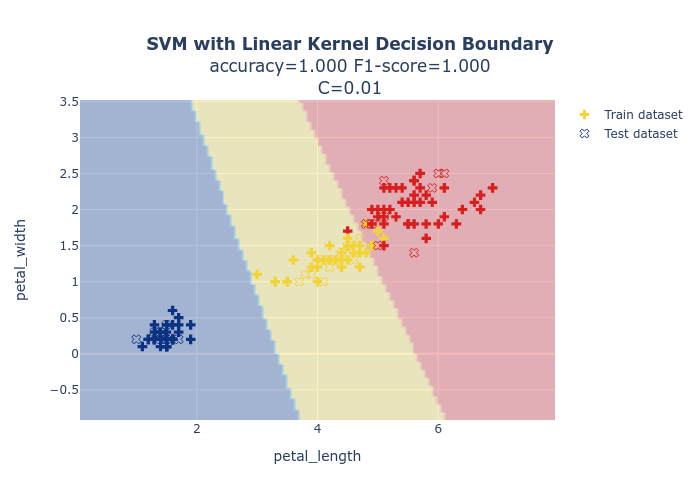
\includegraphics[scale=.13]{images/implementation/q1/linear_kernel/petal_length_petal_width_0.01.png}
    \end{subfigure}
    \hfill
    \begin{subfigure}{0.3\textwidth}
        \centering
        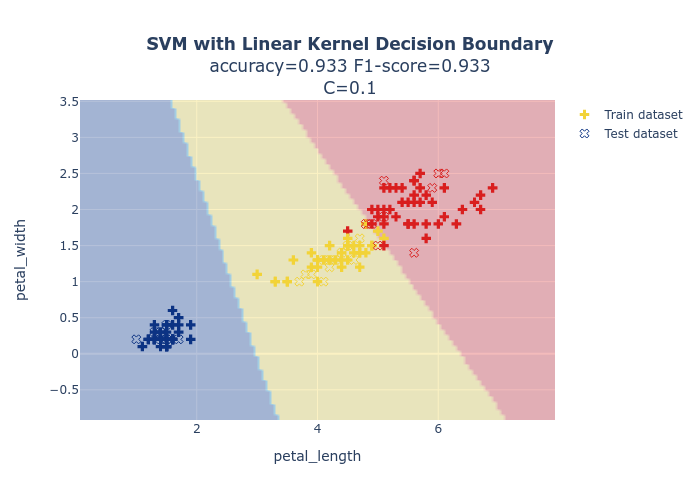
\includegraphics[scale=.13]{images/implementation/q1/linear_kernel/petal_length_petal_width_0.1.png}
    \end{subfigure}
    \hfill
    \begin{subfigure}{0.3\textwidth}
        \centering
        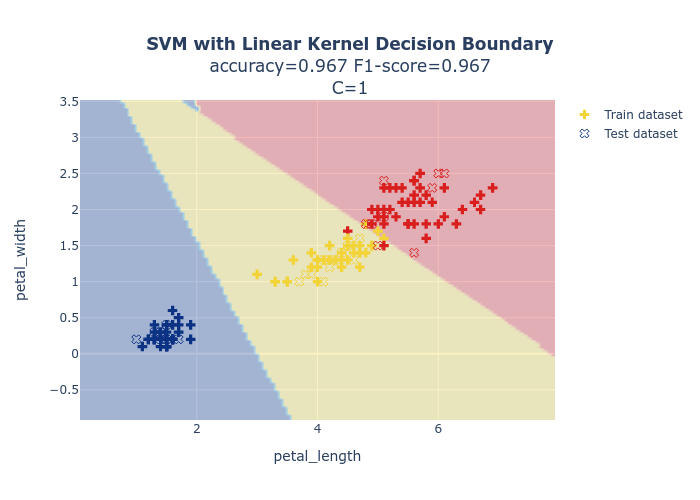
\includegraphics[scale=.13]{images/implementation/q1/linear_kernel/petal_length_petal_width_1.png}
    \end{subfigure}
    \newline
    \begin{subfigure}{0.3\textwidth}
        \centering
        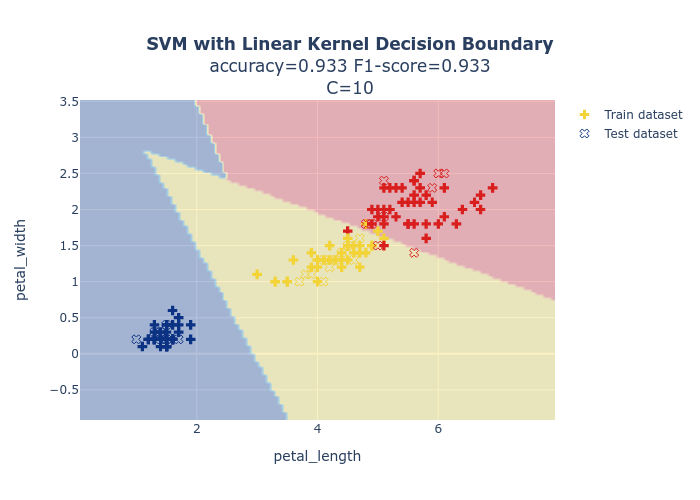
\includegraphics[scale=.13]{images/implementation/q1/linear_kernel/petal_length_petal_width_10.png}
    \end{subfigure}
    \hfill
    \begin{subfigure}{0.3\textwidth}
        \centering
        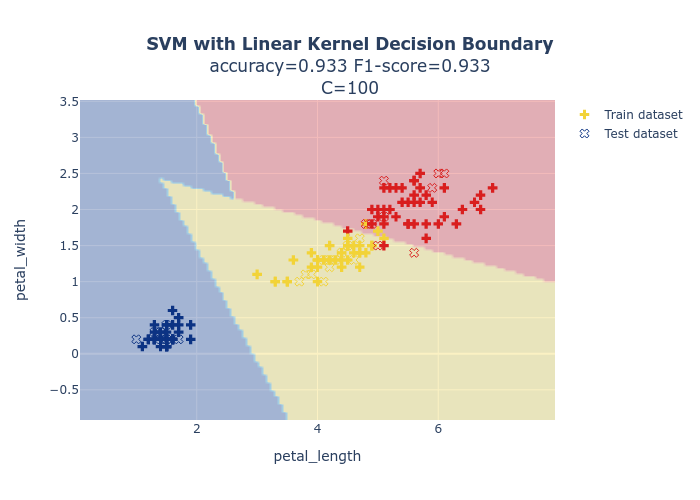
\includegraphics[scale=.13]{images/implementation/q1/linear_kernel/petal_length_petal_width_100.png}
    \end{subfigure}
    \hfill
    \begin{subfigure}{0.3\textwidth}
        \centering
        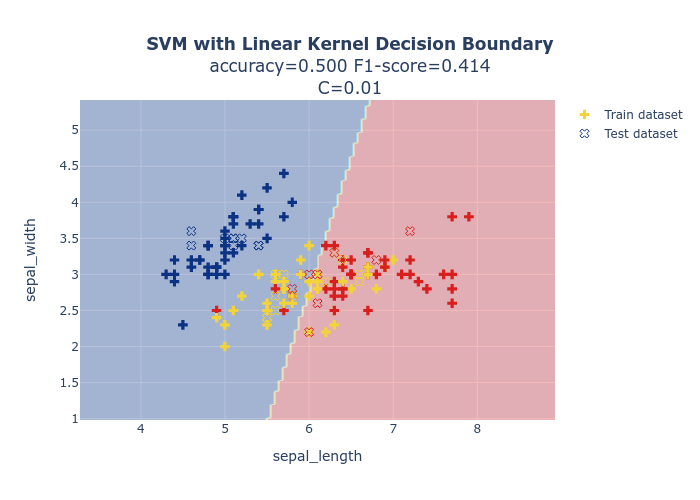
\includegraphics[scale=.13]{images/implementation/q1/linear_kernel/sepal_length_sepal_width_0.01.png}
    \end{subfigure}
    \newline
    \begin{subfigure}{0.3\textwidth}
        \centering
        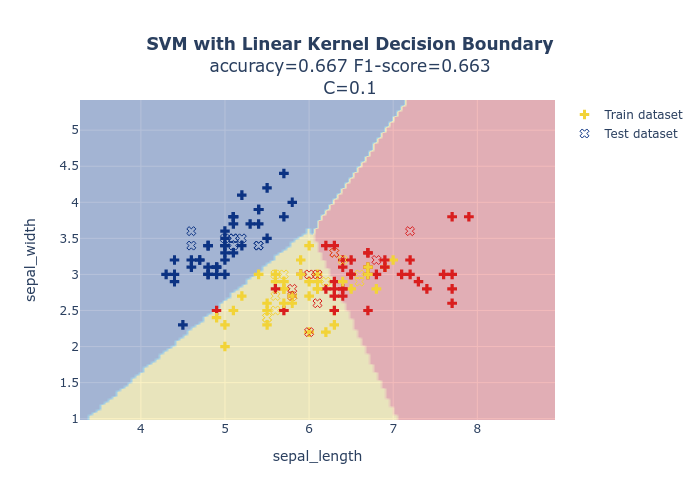
\includegraphics[scale=.13]{images/implementation/q1/linear_kernel/sepal_length_sepal_width_0.1.png}
    \end{subfigure}
    \hfill
    \begin{subfigure}{0.3\textwidth}
        \centering
        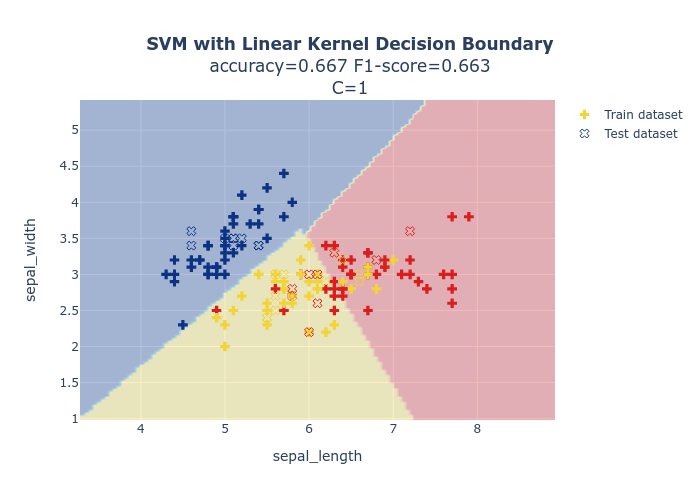
\includegraphics[scale=.13]{images/implementation/q1/linear_kernel/sepal_length_sepal_width_1.png}
    \end{subfigure}
    \hfill
    \begin{subfigure}{0.3\textwidth}
        \centering
        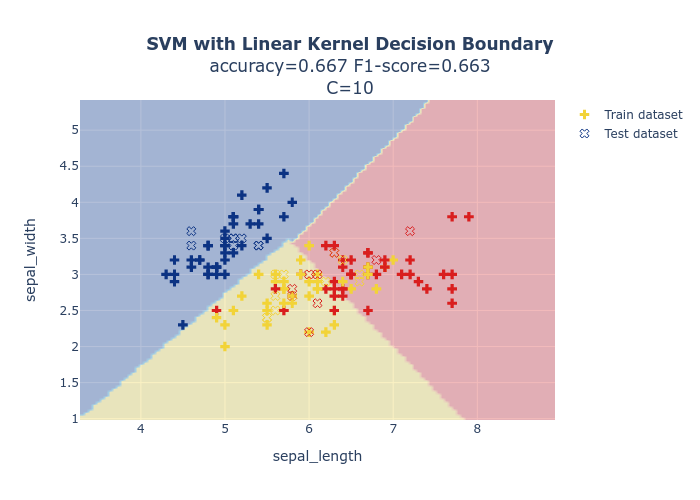
\includegraphics[scale=.13]{images/implementation/q1/linear_kernel/sepal_length_sepal_width_10.png}
    \end{subfigure}
    \newline
    \begin{subfigure}{0.3\textwidth}
        \centering
        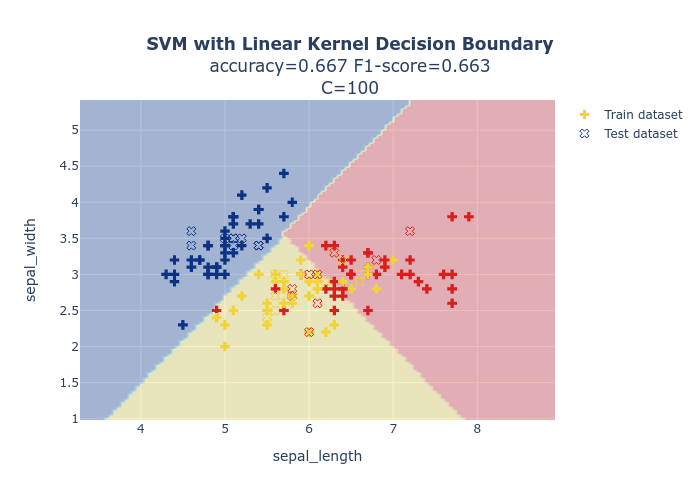
\includegraphics[scale=.13]{images/implementation/q1/linear_kernel/sepal_length_sepal_width_100.png}
    \end{subfigure}
    \caption{دسته‌بندی داده‌های \lr{Iris} با دسته‌بند \lr{SVM} و کرنل خطی}
    \label{linear_kernel}
\end{figure}

\newpage

\begin{figure}
    \begin{subfigure}{0.3\textwidth}
        \centering
        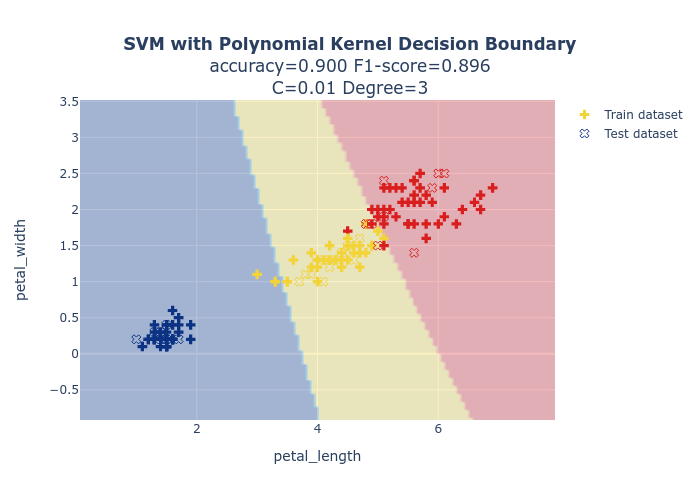
\includegraphics[scale=.13]{images/implementation/q1/polynomial_kernel/petal_length_petal_width_0.01_3.png}
    \end{subfigure}
    \hfill
    \begin{subfigure}{0.3\textwidth}
        \centering
        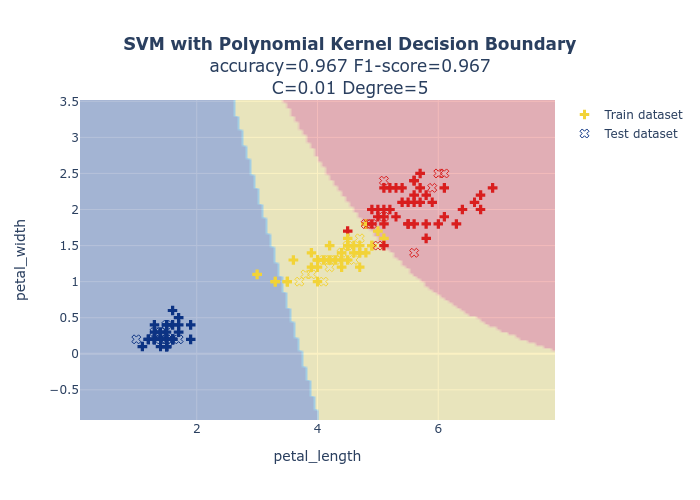
\includegraphics[scale=.13]{images/implementation/q1/polynomial_kernel/petal_length_petal_width_0.01_5.png}
    \end{subfigure}
    \hfill
    \begin{subfigure}{0.3\textwidth}
        \centering
        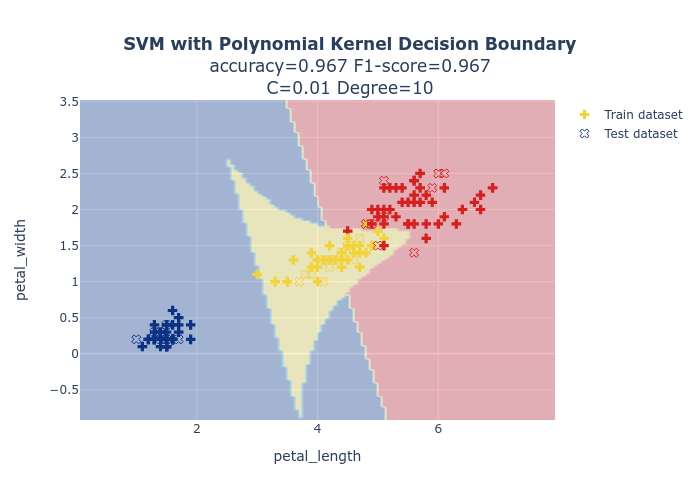
\includegraphics[scale=.13]{images/implementation/q1/polynomial_kernel/petal_length_petal_width_0.01_10.png}
    \end{subfigure}
    \newline
    \begin{subfigure}{0.3\textwidth}
        \centering
        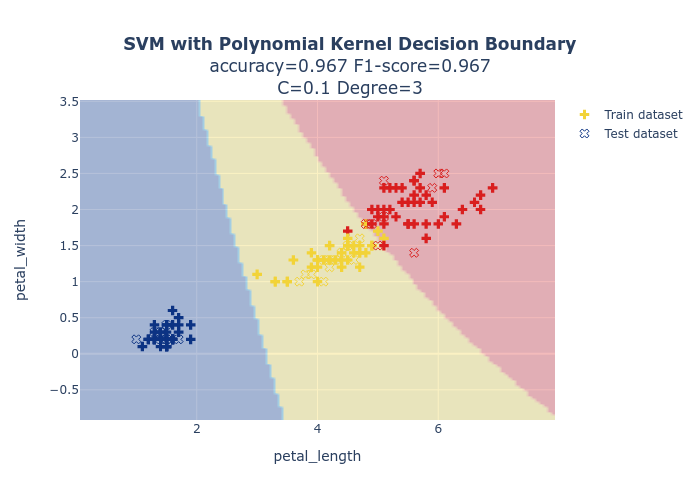
\includegraphics[scale=.13]{images/implementation/q1/polynomial_kernel/petal_length_petal_width_0.1_3.png}
    \end{subfigure}
    \hfill
    \begin{subfigure}{0.3\textwidth}
        \centering
        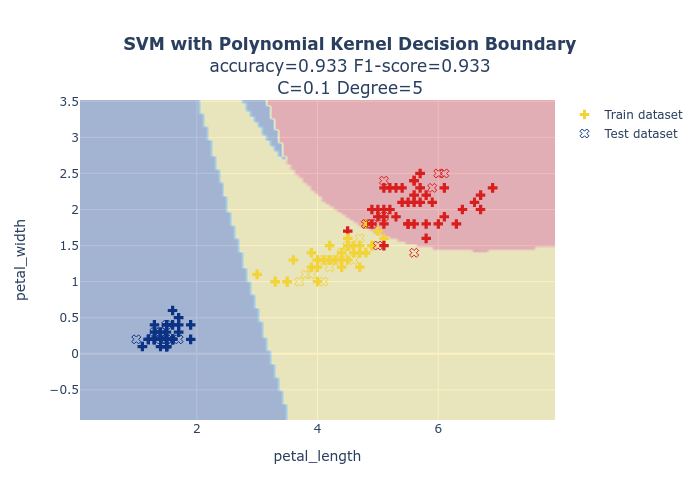
\includegraphics[scale=.13]{images/implementation/q1/polynomial_kernel/petal_length_petal_width_0.1_5.png}
    \end{subfigure}
    \hfill
    \begin{subfigure}{0.3\textwidth}
        \centering
        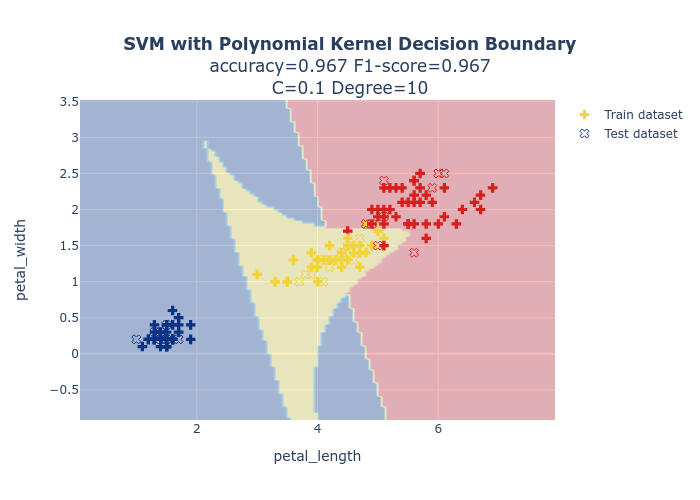
\includegraphics[scale=.13]{images/implementation/q1/polynomial_kernel/petal_length_petal_width_0.1_10.png}
    \end{subfigure}
    \newline
    \begin{subfigure}{0.3\textwidth}
        \centering
        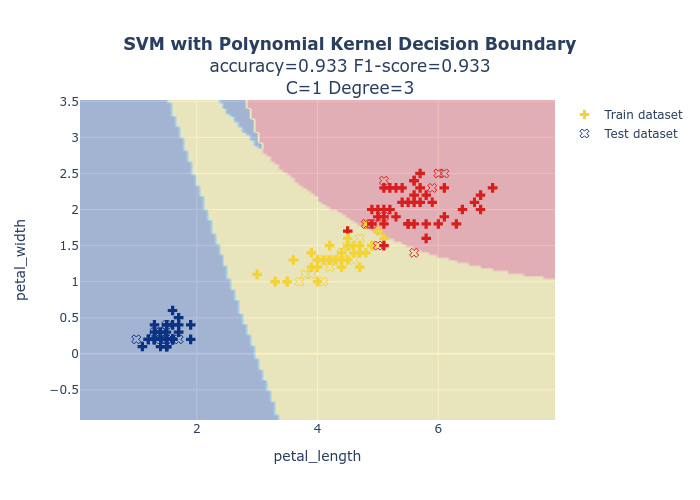
\includegraphics[scale=.13]{images/implementation/q1/polynomial_kernel/petal_length_petal_width_1_3.png}
    \end{subfigure}
    \hfill
    \begin{subfigure}{0.3\textwidth}
        \centering
        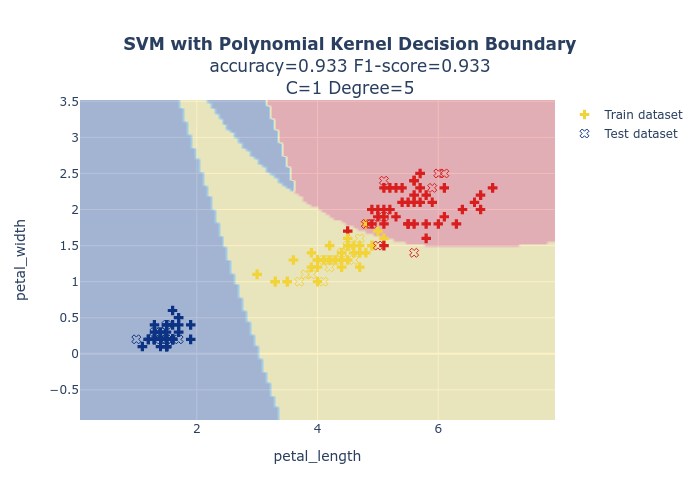
\includegraphics[scale=.13]{images/implementation/q1/polynomial_kernel/petal_length_petal_width_1_5.png}
    \end{subfigure}
    \hfill
    \begin{subfigure}{0.3\textwidth}
        \centering
        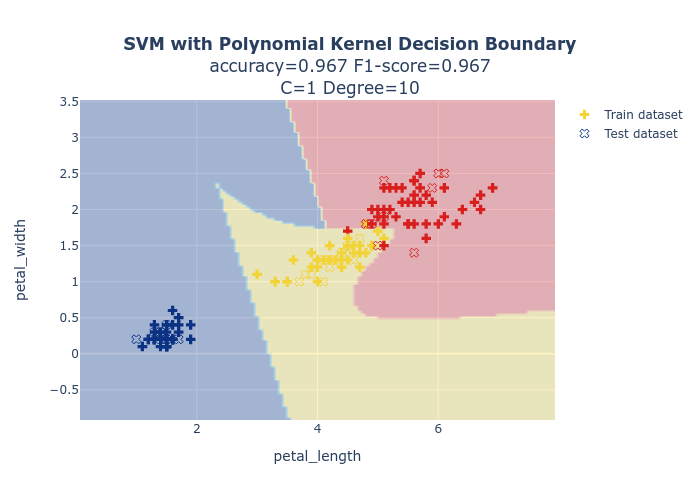
\includegraphics[scale=.13]{images/implementation/q1/polynomial_kernel/petal_length_petal_width_1_10.png}
    \end{subfigure}
    \newline
    \begin{subfigure}{0.3\textwidth}
        \centering
        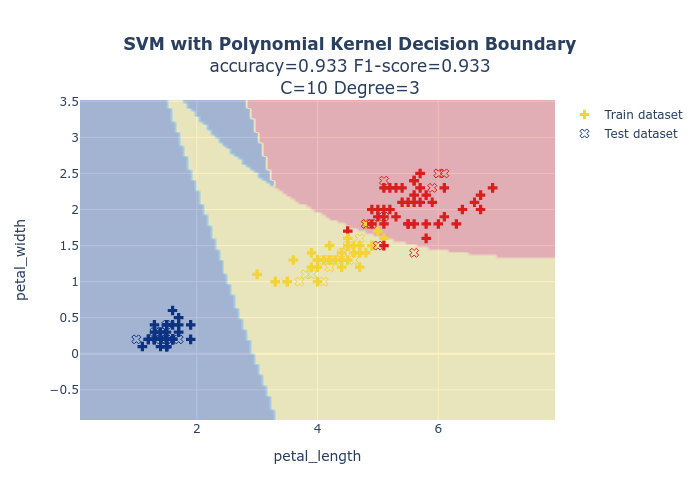
\includegraphics[scale=.13]{images/implementation/q1/polynomial_kernel/petal_length_petal_width_10_3.png}
    \end{subfigure}
    \hfill
    \begin{subfigure}{0.3\textwidth}
        \centering
        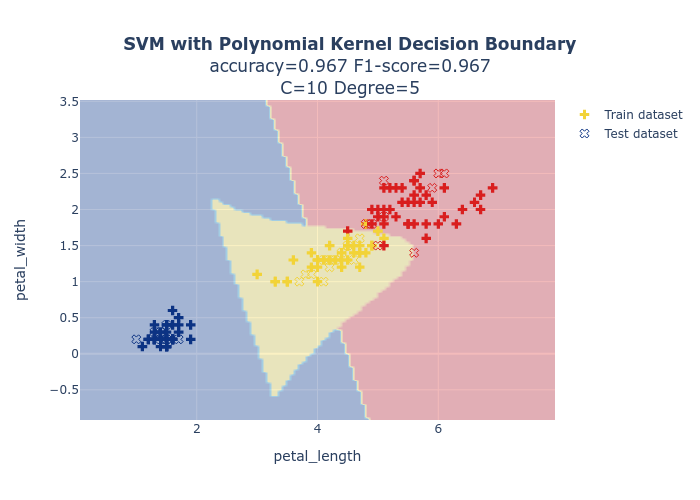
\includegraphics[scale=.13]{images/implementation/q1/polynomial_kernel/petal_length_petal_width_10_5.png}
    \end{subfigure}
    \hfill
    \begin{subfigure}{0.3\textwidth}
        \centering
        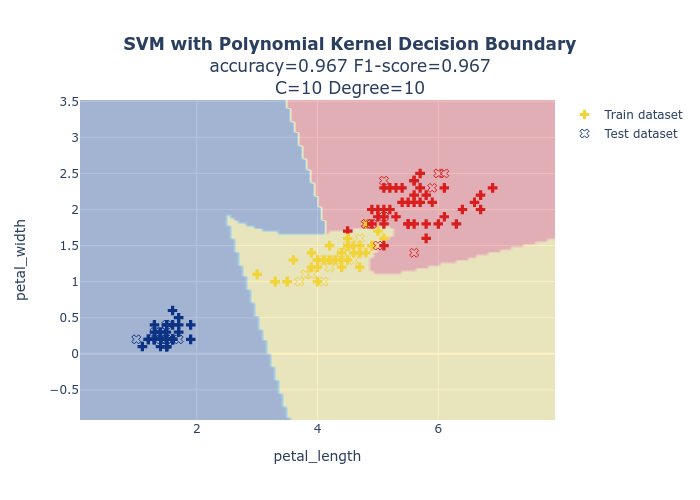
\includegraphics[scale=.13]{images/implementation/q1/polynomial_kernel/petal_length_petal_width_10_10.png}
    \end{subfigure}
    \newline
    \begin{subfigure}{0.3\textwidth}
        \centering
        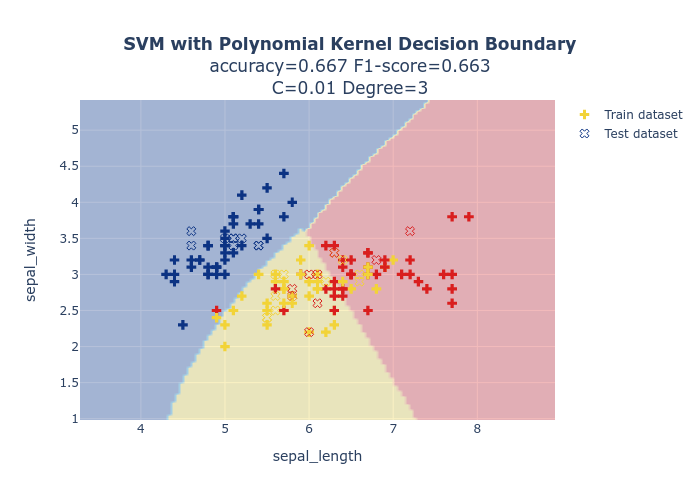
\includegraphics[scale=.13]{images/implementation/q1/polynomial_kernel/sepal_length_sepal_width_0.01_3.png}
    \end{subfigure}
    \hfill
    \begin{subfigure}{0.3\textwidth}
        \centering
        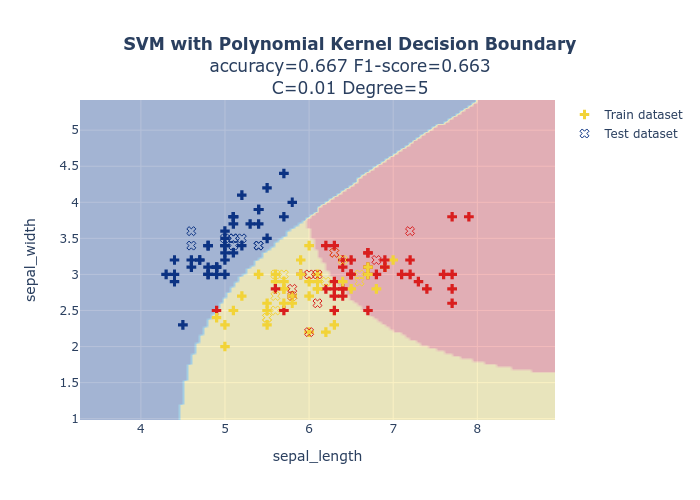
\includegraphics[scale=.13]{images/implementation/q1/polynomial_kernel/sepal_length_sepal_width_0.01_5.png}
    \end{subfigure}
    \hfill
    \begin{subfigure}{0.3\textwidth}
        \centering
        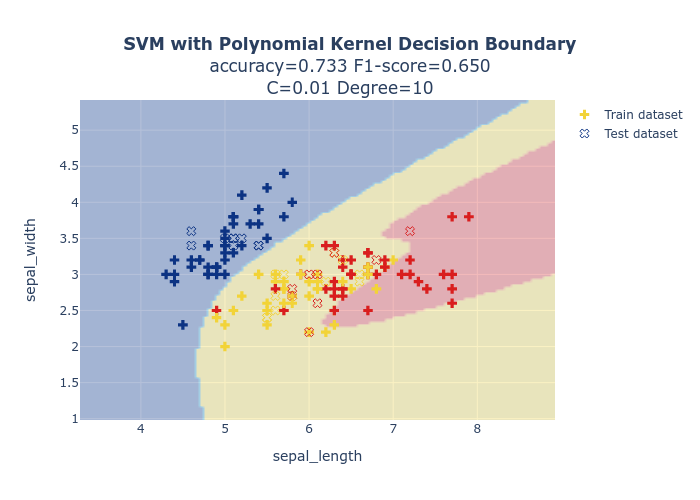
\includegraphics[scale=.13]{images/implementation/q1/polynomial_kernel/sepal_length_sepal_width_0.01_10.png}
    \end{subfigure}
    \newline
    \begin{subfigure}{0.3\textwidth}
        \centering
        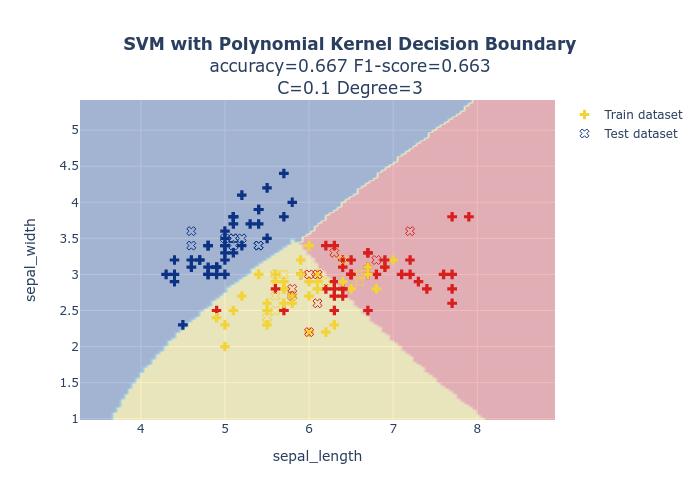
\includegraphics[scale=.13]{images/implementation/q1/polynomial_kernel/sepal_length_sepal_width_0.1_3.png}
    \end{subfigure}
    \hfill
    \begin{subfigure}{0.3\textwidth}
        \centering
        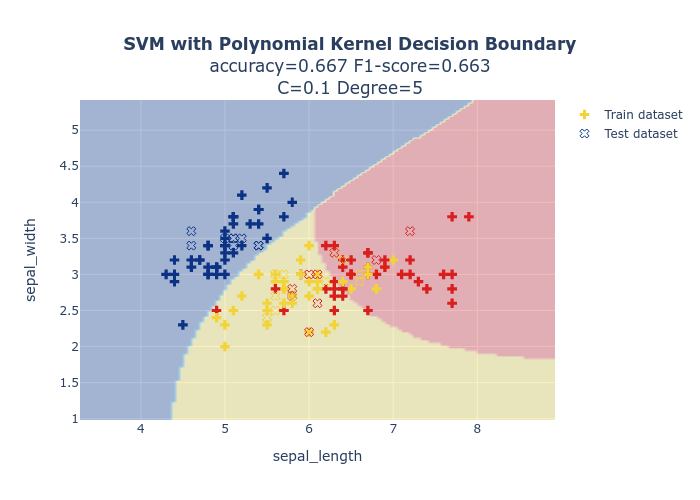
\includegraphics[scale=.13]{images/implementation/q1/polynomial_kernel/sepal_length_sepal_width_0.1_5.png}
    \end{subfigure}
    \hfill
    \begin{subfigure}{0.3\textwidth}
        \centering
        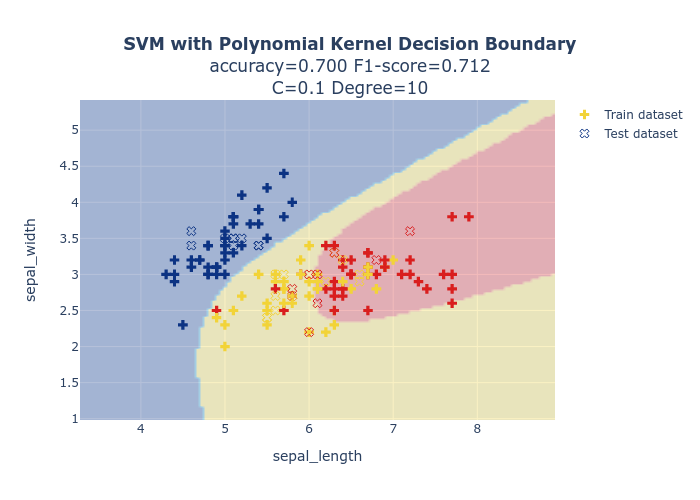
\includegraphics[scale=.13]{images/implementation/q1/polynomial_kernel/sepal_length_sepal_width_0.1_10.png}
    \end{subfigure}
    \newline
    \begin{subfigure}{0.3\textwidth}
        \centering
        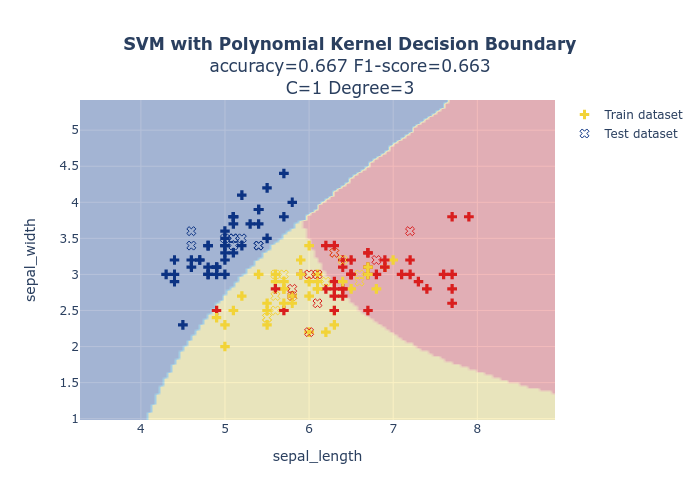
\includegraphics[scale=.13]{images/implementation/q1/polynomial_kernel/sepal_length_sepal_width_1_3.png}
    \end{subfigure}
    \hfill
    \begin{subfigure}{0.3\textwidth}
        \centering
        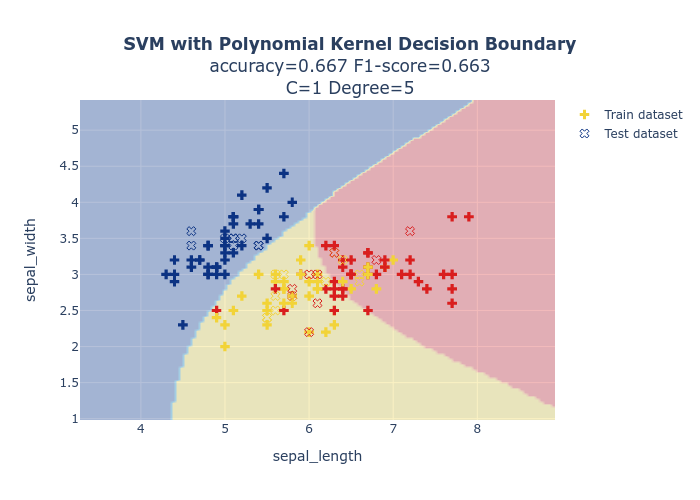
\includegraphics[scale=.13]{images/implementation/q1/polynomial_kernel/sepal_length_sepal_width_1_5.png}
    \end{subfigure}
    \hfill
    \begin{subfigure}{0.3\textwidth}
        \centering
        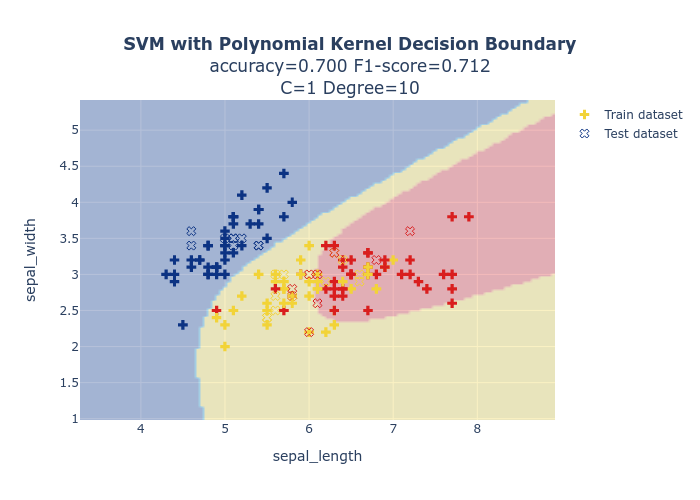
\includegraphics[scale=.13]{images/implementation/q1/polynomial_kernel/sepal_length_sepal_width_1_10.png}
    \end{subfigure}
    \newline
    \begin{subfigure}{0.3\textwidth}
        \centering
        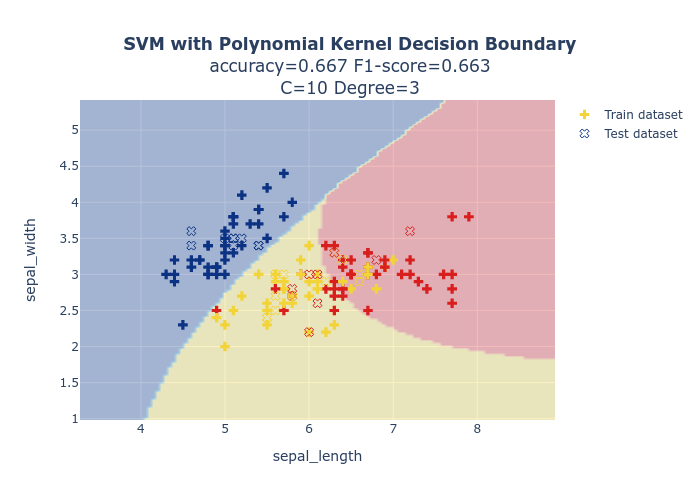
\includegraphics[scale=.13]{images/implementation/q1/polynomial_kernel/sepal_length_sepal_width_10_3.png}
    \end{subfigure}
    \hfill
    \begin{subfigure}{0.3\textwidth}
        \centering
        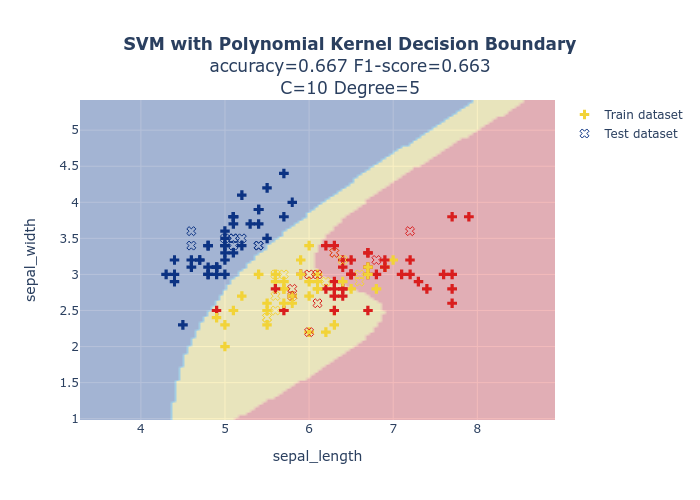
\includegraphics[scale=.13]{images/implementation/q1/polynomial_kernel/sepal_length_sepal_width_10_5.png}
    \end{subfigure}
    \hfill
    \begin{subfigure}{0.3\textwidth}
        \centering
        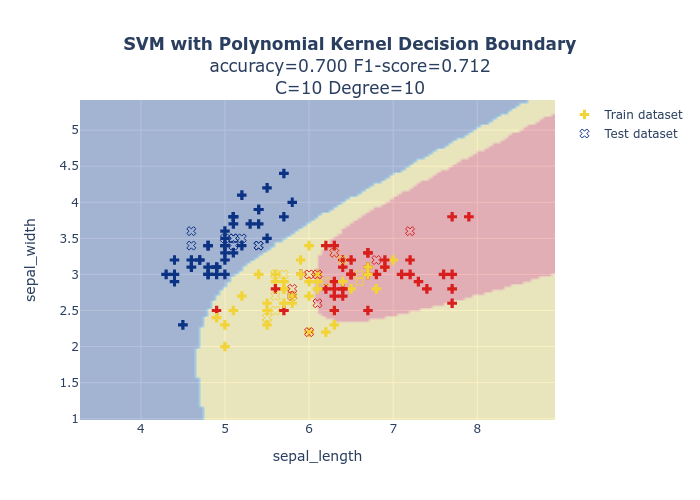
\includegraphics[scale=.13]{images/implementation/q1/polynomial_kernel/sepal_length_sepal_width_10_10.png}
    \end{subfigure}
    \caption{دسته‌بندی داده‌های \lr{Iris} با دسته‌بند \lr{SVM} و کرنل چندجمله‌ای}
    \label{polynomial_kernel}
\end{figure}

\newpage

\begin{figure}
    \begin{subfigure}{0.3\textwidth}
        \centering
        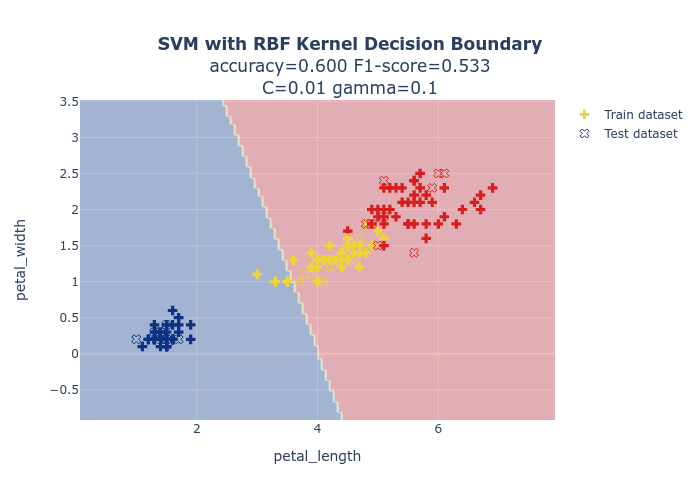
\includegraphics[scale=.13]{images/implementation/q1/rbf_kernel/petal_length_petal_width_0.01_0.1.png}
    \end{subfigure}
    \hfill
    \begin{subfigure}{0.3\textwidth}
        \centering
        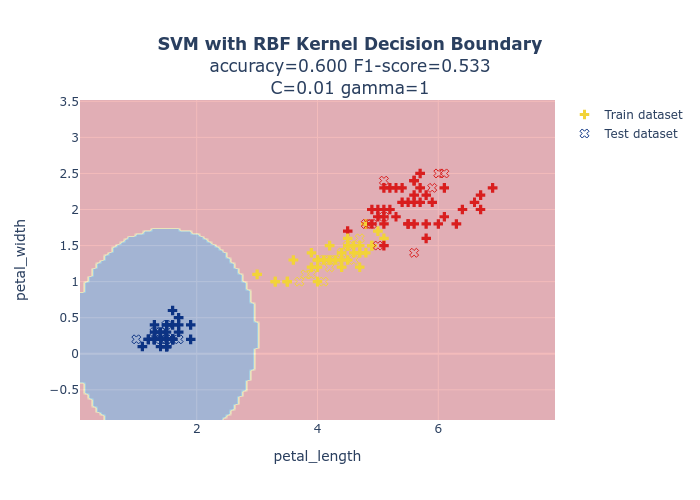
\includegraphics[scale=.13]{images/implementation/q1/rbf_kernel/petal_length_petal_width_0.01_1.png}
    \end{subfigure}
    \hfill
    \begin{subfigure}{0.3\textwidth}
        \centering
        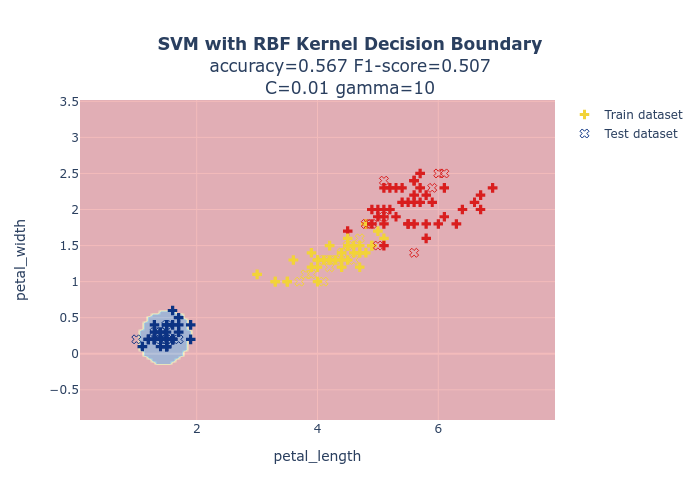
\includegraphics[scale=.13]{images/implementation/q1/rbf_kernel/petal_length_petal_width_0.01_10.png}
    \end{subfigure}
    \newline
    \begin{subfigure}{0.3\textwidth}
        \centering
        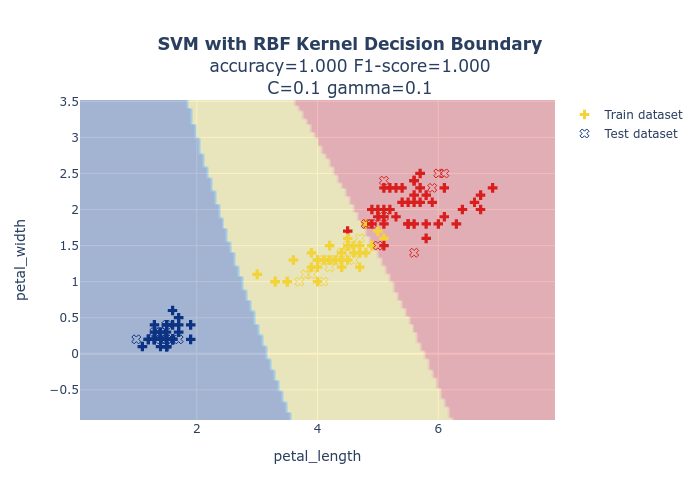
\includegraphics[scale=.13]{images/implementation/q1/rbf_kernel/petal_length_petal_width_0.1_0.1.png}
    \end{subfigure}
    \hfill
    \begin{subfigure}{0.3\textwidth}
        \centering
        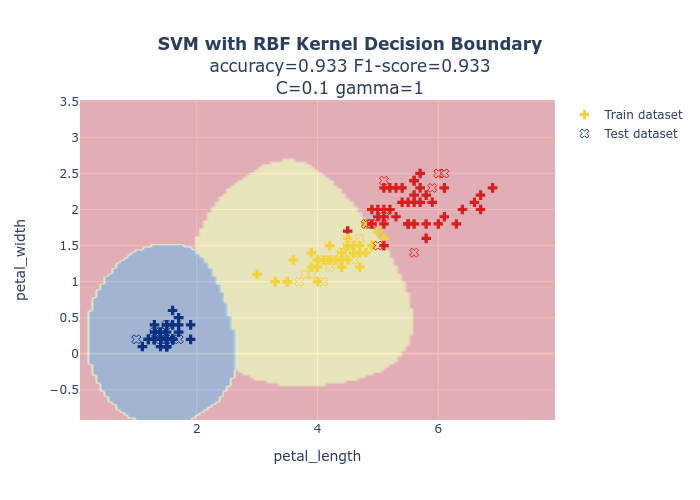
\includegraphics[scale=.13]{images/implementation/q1/rbf_kernel/petal_length_petal_width_0.1_1.png}
    \end{subfigure}
    \hfill
    \begin{subfigure}{0.3\textwidth}
        \centering
        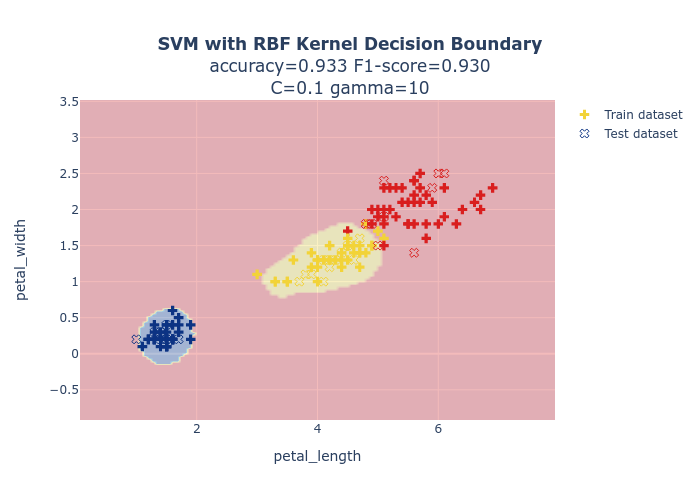
\includegraphics[scale=.13]{images/implementation/q1/rbf_kernel/petal_length_petal_width_0.1_10.png}
    \end{subfigure}
    \newline
    \begin{subfigure}{0.3\textwidth}
        \centering
        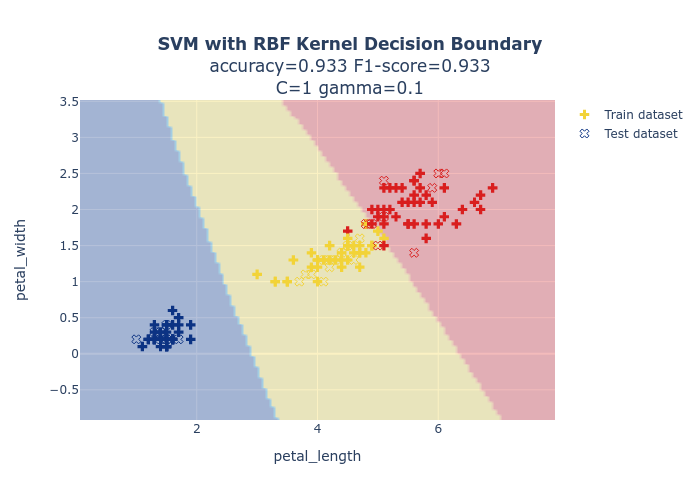
\includegraphics[scale=.13]{images/implementation/q1/rbf_kernel/petal_length_petal_width_1_0.1.png}
    \end{subfigure}
    \hfill
    \begin{subfigure}{0.3\textwidth}
        \centering
        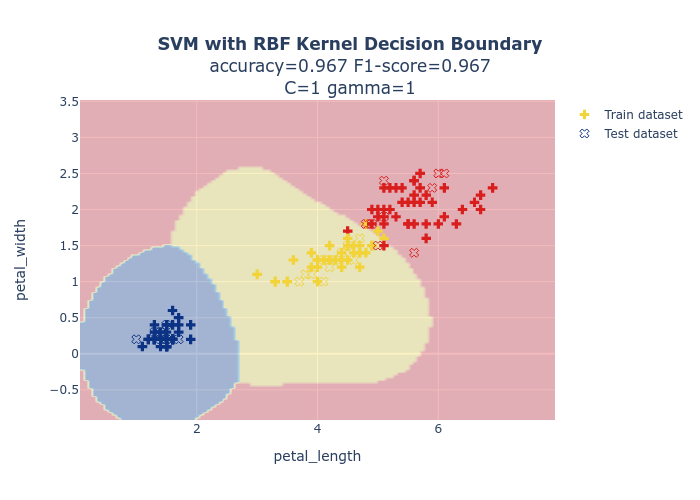
\includegraphics[scale=.13]{images/implementation/q1/rbf_kernel/petal_length_petal_width_1_1.png}
    \end{subfigure}
    \hfill
    \begin{subfigure}{0.3\textwidth}
        \centering
        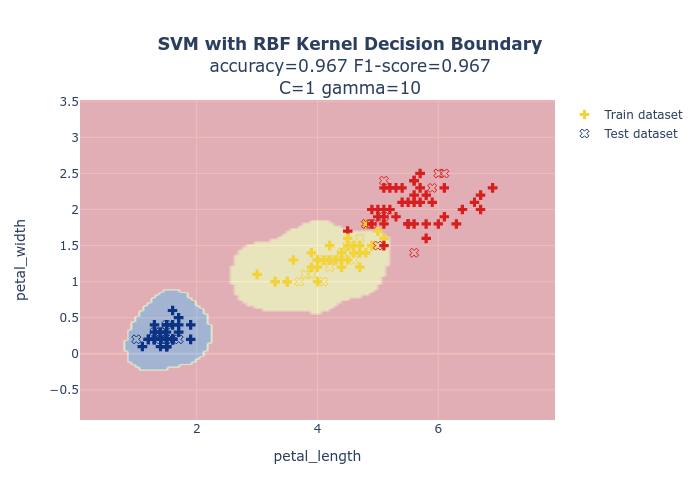
\includegraphics[scale=.13]{images/implementation/q1/rbf_kernel/petal_length_petal_width_1_10.png}
    \end{subfigure}
    \newline
    \begin{subfigure}{0.3\textwidth}
        \centering
        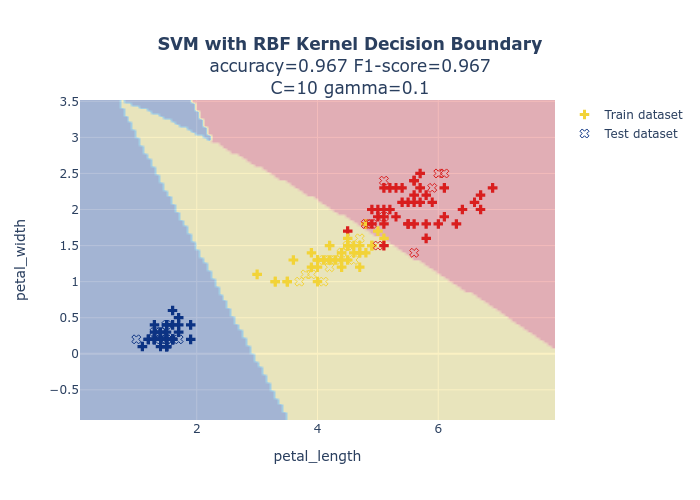
\includegraphics[scale=.13]{images/implementation/q1/rbf_kernel/petal_length_petal_width_10_0.1.png}
    \end{subfigure}
    \hfill
    \begin{subfigure}{0.3\textwidth}
        \centering
        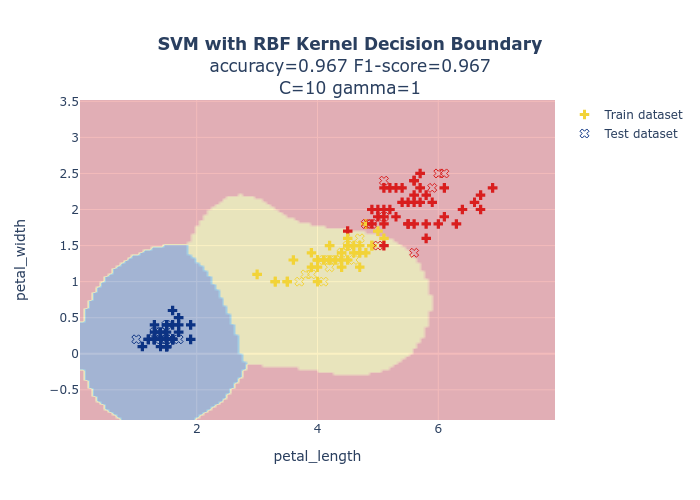
\includegraphics[scale=.13]{images/implementation/q1/rbf_kernel/petal_length_petal_width_10_1.png}
    \end{subfigure}
    \hfill
    \begin{subfigure}{0.3\textwidth}
        \centering
        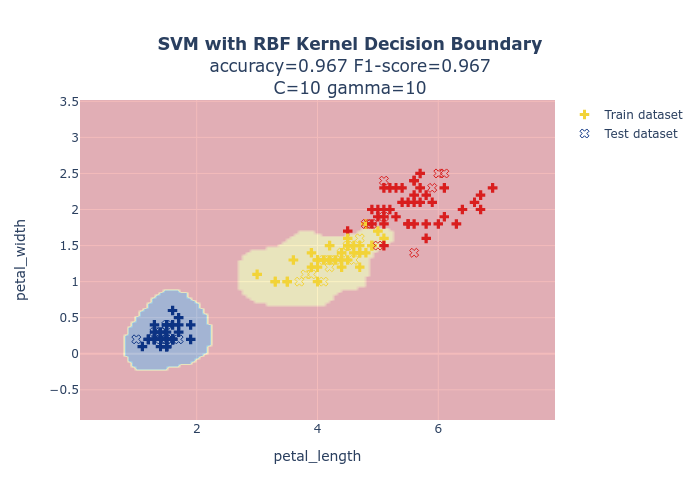
\includegraphics[scale=.13]{images/implementation/q1/rbf_kernel/petal_length_petal_width_10_10.png}
    \end{subfigure}
    \newline
    \begin{subfigure}{0.3\textwidth}
        \centering
        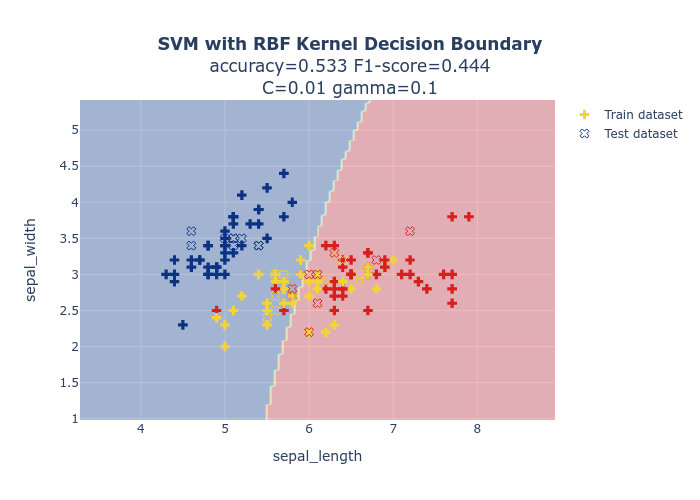
\includegraphics[scale=.13]{images/implementation/q1/rbf_kernel/sepal_length_sepal_width_0.01_0.1.png}
    \end{subfigure}
    \hfill
    \begin{subfigure}{0.3\textwidth}
        \centering
        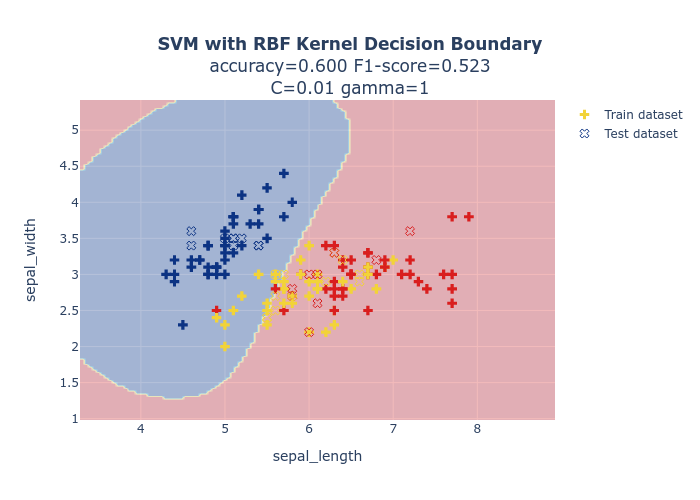
\includegraphics[scale=.13]{images/implementation/q1/rbf_kernel/sepal_length_sepal_width_0.01_1.png}
    \end{subfigure}
    \hfill
    \begin{subfigure}{0.3\textwidth}
        \centering
        \includegraphics[scale=.13]{images/implementation/q1/rbf_kernel/sepal_length_sepal_width_0.01_10.png}
    \end{subfigure}
    \newline
    \begin{subfigure}{0.3\textwidth}
        \centering
        \includegraphics[scale=.13]{images/implementation/q1/rbf_kernel/sepal_length_sepal_width_0.1_0.1.png}
    \end{subfigure}
    \hfill
    \begin{subfigure}{0.3\textwidth}
        \centering
        \includegraphics[scale=.13]{images/implementation/q1/rbf_kernel/sepal_length_sepal_width_0.1_1.png}
    \end{subfigure}
    \hfill
    \begin{subfigure}{0.3\textwidth}
        \centering
        \includegraphics[scale=.13]{images/implementation/q1/rbf_kernel/sepal_length_sepal_width_0.1_10.png}
    \end{subfigure}
    \newline
    \begin{subfigure}{0.3\textwidth}
        \centering
        \includegraphics[scale=.13]{images/implementation/q1/rbf_kernel/sepal_length_sepal_width_1_0.1.png}
    \end{subfigure}
    \hfill
    \begin{subfigure}{0.3\textwidth}
        \centering
        \includegraphics[scale=.13]{images/implementation/q1/rbf_kernel/sepal_length_sepal_width_1_1.png}
    \end{subfigure}
    \hfill
    \begin{subfigure}{0.3\textwidth}
        \centering
        \includegraphics[scale=.13]{images/implementation/q1/rbf_kernel/sepal_length_sepal_width_1_10.png}
    \end{subfigure}
    \newline
    \begin{subfigure}{0.3\textwidth}
        \centering
        \includegraphics[scale=.13]{images/implementation/q1/rbf_kernel/sepal_length_sepal_width_10_0.1.png}
    \end{subfigure}
    \hfill
    \begin{subfigure}{0.3\textwidth}
        \centering
        \includegraphics[scale=.13]{images/implementation/q1/rbf_kernel/sepal_length_sepal_width_10_1.png}
    \end{subfigure}
    \hfill
    \begin{subfigure}{0.3\textwidth}
        \centering
        \includegraphics[scale=.13]{images/implementation/q1/rbf_kernel/sepal_length_sepal_width_10_10.png}
    \end{subfigure}
    \caption{دسته‌بندی داده‌های \lr{Iris} با دسته‌بند \lr{SVM} و کرنل \lr{RBF}}
    \label{rbf_kernel}
\end{figure}

\newpage

\begin{figure}
    \begin{subfigure}{0.3\textwidth}
        \centering
        \includegraphics[scale=.13]{images/implementation/q1/sigmoid_kernel/petal_length_petal_width_0.01_0.001.png}
    \end{subfigure}
    \hfill
    \begin{subfigure}{0.3\textwidth}
        \centering
        \includegraphics[scale=.13]{images/implementation/q1/sigmoid_kernel/petal_length_petal_width_0.01_0.01.png}
    \end{subfigure}
    \hfill
    \begin{subfigure}{0.3\textwidth}
        \centering
        \includegraphics[scale=.13]{images/implementation/q1/sigmoid_kernel/petal_length_petal_width_0.01_0.1.png}
    \end{subfigure}
    \newline
    \begin{subfigure}{0.3\textwidth}
        \centering
        \includegraphics[scale=.13]{images/implementation/q1/sigmoid_kernel/petal_length_petal_width_0.1_0.001.png}
    \end{subfigure}
    \hfill
    \begin{subfigure}{0.3\textwidth}
        \centering
        \includegraphics[scale=.13]{images/implementation/q1/sigmoid_kernel/petal_length_petal_width_0.1_0.01.png}
    \end{subfigure}
    \hfill
    \begin{subfigure}{0.3\textwidth}
        \centering
        \includegraphics[scale=.13]{images/implementation/q1/sigmoid_kernel/petal_length_petal_width_0.1_0.1.png}
    \end{subfigure}
    \newline
    \begin{subfigure}{0.3\textwidth}
        \centering
        \includegraphics[scale=.13]{images/implementation/q1/sigmoid_kernel/petal_length_petal_width_10_0.001.png}
    \end{subfigure}
    \hfill
    \begin{subfigure}{0.3\textwidth}
        \centering
        \includegraphics[scale=.13]{images/implementation/q1/sigmoid_kernel/petal_length_petal_width_10_0.01.png}
    \end{subfigure}
    \hfill
    \begin{subfigure}{0.3\textwidth}
        \centering
        \includegraphics[scale=.13]{images/implementation/q1/sigmoid_kernel/petal_length_petal_width_10_0.1.png}
    \end{subfigure}
    \newline
    \begin{subfigure}{0.3\textwidth}
        \centering
        \includegraphics[scale=.13]{images/implementation/q1/sigmoid_kernel/petal_length_petal_width_100_0.001.png}
    \end{subfigure}
    \hfill
    \begin{subfigure}{0.3\textwidth}
        \centering
        \includegraphics[scale=.13]{images/implementation/q1/sigmoid_kernel/petal_length_petal_width_100_0.01.png}
    \end{subfigure}
    \hfill
    \begin{subfigure}{0.3\textwidth}
        \centering
        \includegraphics[scale=.13]{images/implementation/q1/sigmoid_kernel/petal_length_petal_width_100_0.1.png}
    \end{subfigure}
    \newline
    \begin{subfigure}{0.3\textwidth}
        \centering
        \includegraphics[scale=.13]{images/implementation/q1/sigmoid_kernel/sepal_length_sepal_width_0.01_0.001.png}
    \end{subfigure}
    \hfill
    \begin{subfigure}{0.3\textwidth}
        \centering
        \includegraphics[scale=.13]{images/implementation/q1/sigmoid_kernel/sepal_length_sepal_width_0.01_0.01.png}
    \end{subfigure}
    \hfill
    \begin{subfigure}{0.3\textwidth}
        \centering
        \includegraphics[scale=.13]{images/implementation/q1/sigmoid_kernel/sepal_length_sepal_width_0.01_0.1.png}
    \end{subfigure}
    \newline
    \begin{subfigure}{0.3\textwidth}
        \centering
        \includegraphics[scale=.13]{images/implementation/q1/sigmoid_kernel/sepal_length_sepal_width_0.1_0.001.png}
    \end{subfigure}
    \hfill
    \begin{subfigure}{0.3\textwidth}
        \centering
        \includegraphics[scale=.13]{images/implementation/q1/sigmoid_kernel/sepal_length_sepal_width_0.1_0.01.png}
    \end{subfigure}
    \hfill
    \begin{subfigure}{0.3\textwidth}
        \centering
        \includegraphics[scale=.13]{images/implementation/q1/sigmoid_kernel/sepal_length_sepal_width_0.1_0.1.png}
    \end{subfigure}
    \newline
    \begin{subfigure}{0.3\textwidth}
        \centering
        \includegraphics[scale=.13]{images/implementation/q1/sigmoid_kernel/sepal_length_sepal_width_10_0.001.png}
    \end{subfigure}
    \hfill
    \begin{subfigure}{0.3\textwidth}
        \centering
        \includegraphics[scale=.13]{images/implementation/q1/sigmoid_kernel/sepal_length_sepal_width_10_0.01.png}
    \end{subfigure}
    \hfill
    \begin{subfigure}{0.3\textwidth}
        \centering
        \includegraphics[scale=.13]{images/implementation/q1/sigmoid_kernel/sepal_length_sepal_width_10_0.1.png}
    \end{subfigure}
    \newline
    \begin{subfigure}{0.3\textwidth}
        \centering
        \includegraphics[scale=.13]{images/implementation/q1/sigmoid_kernel/sepal_length_sepal_width_100_0.001.png}
    \end{subfigure}
    \hfill
    \begin{subfigure}{0.3\textwidth}
        \centering
        \includegraphics[scale=.13]{images/implementation/q1/sigmoid_kernel/sepal_length_sepal_width_100_0.01.png}
    \end{subfigure}
    \hfill
    \begin{subfigure}{0.3\textwidth}
        \centering
        \includegraphics[scale=.13]{images/implementation/q1/sigmoid_kernel/sepal_length_sepal_width_100_0.1.png}
    \end{subfigure}
    \caption{دسته‌بندی داده‌های \lr{Iris} با دسته‌بند \lr{SVM} و کرنل \lr{Sigmoid}}
    \label{sigmoid_kernel}
\end{figure}

\end{document}